\chapter{回溯與分支限界}
\label{ch:backtracking}

% 本章的圖共用的樣式（前綴 bt-）
\tikzset{
    bt-n/.style={circle, draw=black!65, minimum size=0.56cm, inner sep=0pt, font=\scriptsize, fill=white},
    bt-dead/.style={bt-n, draw=black!35, text=black!45, dashed, label={[font=\scriptsize, text=black!55, inner sep=1pt]below:$\times$}},
    bt-ans/.style={bt-n, draw=memStroke, very thick, fill=memFill},
    bt-texp/.style={bt-n, draw=coreStroke, thick, fill=coreFill},
    bt-e/.style={draw=black!55},
    bt-el/.style={font=\tiny, inner sep=0.8pt, fill=white, text=black!75},
    bt-num/.style={font=\tiny, text=black!60, inner sep=0.5pt},
    bt-ord/.style={font=\tiny\bfseries, text=coreStroke, inner sep=0.5pt},
    bt-cost/.style={font=\tiny, text=black!80, inner sep=1pt},
    bt-sbox/.style={rectangle, rounded corners=2pt, draw=black!65, font=\tiny, inner sep=1.5pt, minimum width=0.78cm, minimum height=0.42cm, fill=white},
    bt-sans/.style={bt-sbox, draw=memStroke, very thick, fill=memFill},
    bt-kbox/.style={rectangle, rounded corners=2pt, draw=black!65, font=\scriptsize, align=center, inner sep=1.5pt, minimum width=1.05cm, fill=white},
    bt-kexp/.style={bt-kbox, draw=coreStroke, thick, fill=coreFill},
    bt-kdead/.style={bt-kbox, draw=black!35, text=black!50, dashed},
    bt-kbest/.style={bt-kbox, draw=memStroke, very thick, fill=memFill},
    bt-queen/.style={circle, fill=black!80, minimum size=0.2cm, inner sep=0pt},
    bt-gv/.style={circle, draw=black!70, minimum size=0.6cm, inner sep=0pt, font=\small, fill=white},
    bt-ge/.style={draw=black!60, thick},
    bt-lvl/.style={font=\scriptsize, text=black!55, anchor=east},
}
% \btboard{x}{y}{每一列皇后的欄號，0 表示這列還沒放}：左下角在 (x, y) 的 4×4 小棋盤
\newcommand{\btboard}[3]{%
    \begin{scope}[shift={(#1,#2)}]
    \draw[black!45] (0,0) grid[step=0.36] (1.44,1.44);
    \foreach \btc [count=\btr] in {#3} {
        \ifnum\btc>0
            \node[bt-queen] at ({(\btc-0.5)*0.36},{1.44-(\btr-0.5)*0.36}) {};
        \fi
    }
    \end{scope}%
}

社團週末去爬山，小組要從十二樣裝備裡挑一些放進背包，背包最多只能背十三公斤。 每樣裝備
有重量，也有一個大家討論出來的「有用程度」。 把每一種挑法都列出來是 $4096$ 種，一種一
種檢查還不算慢；裝備變成四十樣，就是一兆多種。 一個省事的做法是一樣一樣決定拿或不拿，
決定到一半發現已經超重，後面那幾樣就不必再試。 還能更省嗎？ 假設目前已經裝進去的，加
上「剩下的全部都拿」，有用程度的總和還比不上已經找到的最好組合，後面還要試嗎？ 往下讀
之前，先想想看這兩種「不必再試」各需要知道什麼。

這一章講兩種有系統地搜尋所有可能解的方法。 \textbf{回溯}（backtracking）把一個解看成一
連串的決定，一次做一個決定，發現走不通就退回上一步改試別的；\textbf{分支限界}（branch
and bound）一樣把所有可能畫成一棵樹，但每次挑「看起來最有希望」的節點往下展開，並用上
下界把不可能更好的子樹整棵丟掉。 兩種方法的最壞情況通常都還是指數時間，它們能做的是讓
實際走過的節點少很多。 研究所考試常考的是手算：畫出狀態空間樹、依序標出節點的編號、寫出
分支限界每一步選了哪個節點、算出界限。 這一章的例子都照這個方式一步一步寫出來。

這一章用到《C 程式設計基礎》第~15~章的遞迴與回溯、第~19~章的 \texttt{malloc}、
\texttt{free}；分支限界的優先佇列用第~8~章的堆積，佇列與堆疊見第~6~章。 0/1 背包的動態規
劃在第~18~章，分數背包的貪心解在第~19~章，這一章會用到後者當作上界。

\section{狀態空間樹與回溯}
\label{sec:bk-tree}

\begin{cbookrecap}[第~15~章 15.15 節]
回溯的程式有固定的形狀：在每一層列出所有可以做的選擇，對每一個選擇先「做」，再遞迴往下
「探索」，回來之後「撤銷」，然後試下一個選擇。 狀態如果用參數傳值（例如還要湊的和
$k$），子呼叫回來時呼叫的人手上的值沒有變，不必另外撤銷；狀態如果是同一塊被就地修改的陣
列（例如棋盤），回來時一定要把改過的格子還原。 那一節寫過三個例子：數有幾個子集合的和是
$k$、數 $n$ 皇后有幾組解、用交換產生所有排列。 這一章不再重講這些程式怎麼寫，重點放在
「搜尋的是哪一棵樹」以及「哪些節點可以不走」。
\end{cbookrecap}

\subsection{解向量、限制與狀態空間樹}

很多問題的答案可以寫成一個向量 $(x_1, x_2, \ldots, x_n)$，每一個 $x_i$ 從一個有限的集合
$S_i$ 裡挑。 例如 $n$ 皇后問題（在 $n \times n$ 的棋盤上放 $n$ 個皇后，任兩個不在同一
列、同一欄或同一條對角線上），可以讓 $x_i$ 表示第 $i$ 列的皇后放在第幾欄。 每一列一定恰
好一個皇后，所以這樣寫不會漏掉任何解。

問題的條件分成兩種：

\begin{itemize}
\item \textbf{顯式限制}（explicit constraint）規定每一個 $x_i$ 能取哪些值，也就是 $S_i$。
例如 $x_i \in \{1, 2, \ldots, n\}$。
\item \textbf{隱式限制}（implicit constraint）規定各個 $x_i$ 之間的關係。 例如任兩個皇后不
同欄（$x_i \ne x_j$），也不在同一條對角線（$|x_i - x_j| \ne |i - j|$）。
\end{itemize}

同一個問題可以把不同的條件放在顯式限制裡。 把「不同欄」也算成顯式限制，$(x_1, \ldots,
x_n)$ 就必須是 $1, \ldots, n$ 的一個排列，要搜尋的可能性從 $n^n$ 種降到 $n!$ 種。

把所有可能的向量組織成一棵樹，叫做\textbf{狀態空間樹}（state space tree）。 根代表什麼都
還沒決定；深度 $k$ 的節點代表已經決定好 $x_1, \ldots, x_k$；一個節點的子節點對應 $x_{k+1}$
的每一個可能值。 樹上的名詞：

\begin{itemize}
\item 每一個節點都是一個\textbf{問題狀態}（problem state）。
\item 從根到某個節點的路徑如果已經是一個滿足顯式限制的完整向量，這個節點是
\textbf{解狀態}（solution state）；向量長度固定為 $n$ 時，解狀態就是深度 $n$ 的葉節點。
\item 解狀態如果也滿足隱式限制，叫做\textbf{答案狀態}（answer state），也叫答案節點。
\end{itemize}

$4$ 皇后的狀態空間樹，如果每一列都允許 $4$ 個欄位，有 $1 + 4 + 4^2 + 4^3 + 4^4 = 341$ 個
節點；用排列樹（同一條路徑上的欄號不重複），只剩 $1 + 4 + 4 \cdot 3 + 4 \cdot 3 \cdot 2 +
4! = 65$ 個節點。 這一章的 $n$ 皇后一律用排列樹。

搜尋時要追蹤每個節點的狀況：

\begin{itemize}
\item \textbf{活節點}（live node）：已經產生出來、但子節點還沒有全部產生的節點。
\item \textbf{E-節點}（E-node，expansion node，擴展節點）：目前正在產生子節點的那一個活節點。
\item \textbf{死節點}（dead node）：被判定不必再展開，或子節點已經全部產生完的節點。
\end{itemize}

判定一個節點不必展開的依據叫做\textbf{界限函數}（bounding function）：給定
$x_1, \ldots, x_k$，如果可以確定它不管怎麼往下補都不會成為答案，界限函數就回答「否」，這
個節點直接變成死節點，整棵子樹都不走。 這個動作叫做\textbf{剪枝}（pruning）。

\textbf{回溯}就是用深度優先的順序走狀態空間樹，邊走邊產生節點，並用界限函數剪枝。 一個
節點一產生出來，只要沒有被剪掉，就馬上變成新的 E-節點，原來的 E-節點要等這個子節點的子樹
走完才繼續產生下一個子節點。 第~\ref{sec:bk-bb}~節的分支限界則是讓一個 E-節點一次把子節點
全部產生完，再從活節點裡挑下一個 E-節點。 兩種方法搜尋的是同一棵樹，差別在節點展開的順
序。

\begin{pseudo}[label=alg:bk-generic, unbreakable]{回溯的骨架}
\Procedure{Backtrack}{$k$}
    \For{$x_k$ 的每一個候選值 $c$，依固定的順序}
        \If{\Call{Promising}{$x_1, \ldots, x_{k-1}, c$}}
            \State $x_k \gets c$
            \If{$(x_1, \ldots, x_k)$ 是答案}
                \State 輸出 $(x_1, \ldots, x_k)$
            \EndIf
            \If{$k < n$}
                \State \Call{Backtrack}{$k + 1$}
            \EndIf
        \EndIf
    \EndFor
\EndProcedure
\end{pseudo}

第 3 行的 \proc{Promising} 就是界限函數，回傳 \TRUE{} 表示這個節點還有希望。 呼叫
\proc{Backtrack}$(1)$ 開始搜尋。 只要一組答案時，在第 6 行找到答案後設一個旗標，讓所有
呼叫都提早結束。 回溯法的時間大約是「產生的節點數 $\times$ 每個節點的成本」；每個節點的
成本主要是第 3 行，節點數則要看界限函數剪掉多少，很難事先算準。

\subsection{\texorpdfstring{$n$}{n} 皇后}
\label{sec:bk-queens}

第 $k$ 列要把皇后放在第 $c$ 欄時，要檢查前面 $k - 1$ 列的皇后。 同一欄的檢查交給排列
樹：已經用過的欄不算子節點。 對角線的檢查有兩種寫法。 直接的寫法是逐一檢查 $i = 1, \ldots,
k - 1$ 是否 $|x_i - c| = k - i$，每個節點花 $O(k)$。 另一種寫法注意到同一條「左下到右上」
的對角線上，列號加欄號是定值；同一條「左上到右下」的對角線上，列號減欄號是定值。 用兩個
布林陣列記錄每一條對角線有沒有皇后，每個節點只要 $O(1)$：

\begin{pseudo}[label=alg:bk-queens]{$n$ 皇后（排列樹，用陣列檢查）}
\Procedure{Queens}{$k$}
    \For{$c \gets 1$ \To $n$}
        \If{$\mathit{col}[c] = \FALSE$} \Comment{排列樹：用過的欄不是子節點}
            \If{$d_1[k + c] = \FALSE$ \AND $d_2[k - c + n] = \FALSE$}
                \State $x_k \gets c$
                \State $\mathit{col}[c] \gets d_1[k + c] \gets d_2[k - c + n] \gets \TRUE$
                \If{$k = n$}
                    \State 輸出 $(x_1, \ldots, x_n)$
                \Else
                    \State \Call{Queens}{$k + 1$}
                \EndIf
                \State $\mathit{col}[c] \gets d_1[k + c] \gets d_2[k - c + n] \gets \FALSE$
            \EndIf
        \EndIf
    \EndFor
\EndProcedure
\end{pseudo}

$k + c$ 的範圍是 $2$ 到 $2n$，$k - c + n$ 的範圍是 $1$ 到 $2n - 1$，所以兩個對角線陣列各
要 $2n - 1$ 格（$d_1$ 從 $2$ 開始編號）。 第 11 行是撤銷：這三個陣列是所有遞迴呼叫共用的，
不還原的話，下一個候選值看到的是上一條分支留下的記號。

\subsubsection{4 皇后的狀態空間樹}

圖~\ref{fig:bk-4queens} 是 \proc{Queens}$(1)$ 在 $n = 4$ 時，找到第一組解之前產生的所有節
點。 節點裡的數字是產生的順序（根是 $1$），邊上的數字是這一列的皇后放在第幾欄。 虛線節點
上打叉的，是第 4 行的對角線檢查沒有通過、產生之後馬上變成死節點的節點；橘色是答案節點。

\begin{center}
\begin{tikzpicture}[x=1.35cm,y=1.05cm]
\node[bt-n] (q1) at (3.681,0.0) {1};
\node[bt-n] (q2) at (1.662,-1.05) {2};
\node[bt-dead] (q3) at (0.0,-2.1) {3};
\node[bt-n] (q4) at (1.425,-2.1) {4};
\node[bt-dead] (q5) at (0.95,-3.15) {5};
\node[bt-dead] (q6) at (1.9,-3.15) {6};
\node[bt-n] (q7) at (3.325,-2.1) {7};
\node[bt-n] (q8) at (2.85,-3.15) {8};
\node[bt-dead] (q9) at (2.85,-4.2) {9};
\node[bt-dead] (q10) at (3.8,-3.15) {10};
\node[bt-n] (q11) at (5.7,-1.05) {11};
\node[bt-dead] (q12) at (4.75,-2.1) {12};
\node[bt-dead] (q13) at (5.7,-2.1) {13};
\node[bt-n] (q14) at (6.65,-2.1) {14};
\node[bt-n] (q15) at (6.65,-3.15) {15};
\node[bt-ans] (q16) at (6.65,-4.2) {16};
\draw[bt-e] (q1) -- node[bt-el] {1} (q2);
\draw[bt-e] (q2) -- node[bt-el] {2} (q3);
\draw[bt-e] (q2) -- node[bt-el] {3} (q4);
\draw[bt-e] (q4) -- node[bt-el] {2} (q5);
\draw[bt-e] (q4) -- node[bt-el] {4} (q6);
\draw[bt-e] (q2) -- node[bt-el] {4} (q7);
\draw[bt-e] (q7) -- node[bt-el] {2} (q8);
\draw[bt-e] (q8) -- node[bt-el] {3} (q9);
\draw[bt-e] (q7) -- node[bt-el] {3} (q10);
\draw[bt-e] (q1) -- node[bt-el] {2} (q11);
\draw[bt-e] (q11) -- node[bt-el] {1} (q12);
\draw[bt-e] (q11) -- node[bt-el] {3} (q13);
\draw[bt-e] (q11) -- node[bt-el] {4} (q14);
\draw[bt-e] (q14) -- node[bt-el] {1} (q15);
\draw[bt-e] (q15) -- node[bt-el] {3} (q16);

\node[bt-lvl] at (-0.4,-1.05) {第 1 列};
\node[bt-lvl] at (-0.4,-2.10) {第 2 列};
\node[bt-lvl] at (-0.4,-3.15) {第 3 列};
\node[bt-lvl] at (-0.4,-4.20) {第 4 列};
\end{tikzpicture}
\diagcaption{4 皇后的回溯，到找到第一組解為止。 節點內是產生的順序，邊上是皇后所在的欄，
左邊標的是這一層決定第幾列。 打叉的節點被對角線檢查剪掉。}
\label{fig:bk-4queens}
\end{center}

照產生的順序讀一遍：

\begin{enumerate}
\item 節點 2：第 1 列放第 1 欄。 第 1 列沒有別的皇后要檢查，一定通過。
\item 節點 3：第 2 列放第 2 欄，和 $(1, 1)$ 在同一條對角線上，剪掉。 節點 4：第 2 列放第
3 欄，通過。
\item 節點 5、6：第 3 列只剩第 2、4 欄可以試。 第 2 欄和 $(2, 3)$ 同一條對角線，第 4 欄
也和 $(2, 3)$ 同一條對角線，兩個都剪掉。 節點 4 的子節點全部是死節點，退回節點 2。
\item 節點 7：第 2 列放第 4 欄。 節點 8：第 3 列放第 2 欄，通過。 節點 9：第 4 列只剩第 3
欄，和 $(3, 2)$ 同一條對角線，剪掉，退回節點 7。 節點 10：第 3 列放第 3 欄，和 $(2, 4)$
同一條對角線，剪掉。 節點 7、節點 2 的子節點都試完了，退回根。
\item 節點 11：第 1 列放第 2 欄。 節點 12（第 1 欄）、13（第 3 欄）都和 $(1, 2)$ 同一條對
角線。 節點 14：第 4 欄，通過。 節點 15：第 3 列放第 1 欄，通過。 節點 16：第 4 列放第 3
欄，通過，得到答案 $(2, 4, 1, 3)$。
\end{enumerate}

一共產生 $16$ 個節點，其中 $7$ 個被剪掉。 排列樹本來有 $65$ 個節點，第一組解在整棵樹裡是
用深度優先順序數過來的第 $31$ 個節點，前面那些子樹大多沒有走到。 圖~\ref{fig:bk-boards}
是節點 4 走不下去和節點 16 找到答案時的棋盤。

\begin{center}
\begin{tikzpicture}
\btboard{0}{0}{1,3,0,0}
\node[font=\footnotesize] at (0.72,-0.35) {節點 4：第 3 列無處可放};
\btboard{4.6}{0}{1,4,2,0}
\node[font=\footnotesize] at (5.32,-0.35) {節點 8：第 4 列無處可放};
\btboard{9.2}{0}{2,4,1,3}
\node[font=\footnotesize] at (9.92,-0.35) {節點 16：答案 $(2, 4, 1, 3)$};
\end{tikzpicture}
\diagcaption{三個時間點的棋盤。 前兩個是死路，最後一個是第一組解。}
\label{fig:bk-boards}
\end{center}

\begin{examnote}
畫狀態空間樹的題目，先看清楚題目用的是哪一種樹（每列 $n$ 個子節點，還是排列樹），以及節點
怎麼編號。 本書用「產生的順序」編號，被剪掉的節點也編號，並畫出來打叉；有些課本改用整棵
排列樹的深度優先編號，同一個答案節點在那種編法裡是第 $31$ 號；也有課本只畫通過檢查的節
點。 欄位一律從小到大試。 題目沒有規定時，寫一句你用的編號方式，畫到題目要求的地方（通常
是第一組解）為止。
\end{examnote}

\subsubsection{C 程式}

下面的程式對輸入的每一個 $n$ 做完整的搜尋，數出解的個數和產生的節點數（包括根和被剪掉的
節點），並記下第一組解是第幾個產生的節點。 搜尋要用到的陣列放在一個結構裡，用指標傳給遞
迴函式，所以程式裡沒有全域變數。

\begin{example}[label=ex:bk-nqueens]{c}{(nqueens.c) $n$ 皇后：計數並印出第一組解}
#include <stdio.h>
#include <stdlib.h>

// 搜尋狀態：第 r 列的皇后在第 col[r] 欄（從 0 起算）
typedef struct {
    int n, *col, *first;
    char *used, *d1, *d2;       // 欄、兩個方向的對角線有沒有皇后
    long long nodes, solutions, first_at;
} Search;

static void place(Search *s, int r)
{
    int n = s->n;
    for (int c = 0; c < n; c++) {
        if (s->used[c]) {
            continue;               // 排列樹裡沒有這個子節點
        }
        s->nodes++;                 // 產生節點 (r, c)
        if (s->d1[r + c] || s->d2[r - c + n - 1]) {
            continue;               // 對角線上已經有皇后：剪掉
        }
        s->col[r] = c;
        s->used[c] = s->d1[r + c] = s->d2[r - c + n - 1] = 1;
        if (r < n - 1) {
            place(s, r + 1);
        } else if (s->solutions++ == 0) {   // 第一組解：記下來
            for (int i = 0; i < n; i++) {
                s->first[i] = s->col[i];
            }
            s->first_at = s->nodes;
        }
        // 撤銷
        s->used[c] = s->d1[r + c] = s->d2[r - c + n - 1] = 0;
    }
}

int main(void)
{
    int n;
    while (scanf("%d", &n) == 1 && n >= 1 && n <= 16) {
        Search s = {n, malloc(n * sizeof(int)),
                    malloc(n * sizeof(int)), calloc(n, 1),
                    calloc(2 * n - 1, 1), calloc(2 * n - 1, 1),
                    1, 0, 0};
        if (s.col && s.first && s.used && s.d1 && s.d2) {
            place(&s, 0);
            printf("n = %d: %lld solutions, %lld nodes\n",
                   n, s.solutions, s.nodes);
            if (s.solutions > 0) {
                printf("first at node %lld:", s.first_at);
                for (int i = 0; i < n; i++) {
                    printf(" %d", s.first[i] + 1);  // 欄號從 1 起算
                }
                printf("\n");
            }
        }
        free(s.col); free(s.first); free(s.used);
        free(s.d1); free(s.d2);
    }
    return 0;
}
\end{example}
\iosample{4 8}{n = 4: 2 solutions, 33 nodes \\ first at node 16: 2 4 1 3 \\ n = 8: 92 solutions, 5509 nodes \\ first at node 337: 1 5 8 6 3 7 2 4}

$n = 4$ 第一組解在第 $16$ 個節點，和圖~\ref{fig:bk-4queens} 一致；搜尋完整棵樹一共產生
$33$ 個節點，找到 $2$ 組解。 下表把 $n = 4$ 到 $8$ 的節點數和兩種狀態空間樹的大小放在一
起（中間幾列用同一支程式輸入 \texttt{5 6 7} 得到）。 界限函數剪掉的比例隨著 $n$ 變大越來
越高：$n = 8$ 時排列樹有十萬多個節點，實際只產生 $5509$ 個。

\begin{center}
\begin{tabular}{crrrr}
\toprule
$n$ & 解的個數 & 回溯產生的節點 & 排列樹的節點 & 每列 $n$ 個子節點的樹 \\
\midrule
4 & 2 & 33 & 65 & 341 \\
5 & 10 & 102 & 326 & 3906 \\
6 & 4 & 357 & 1957 & 55987 \\
7 & 40 & 1346 & 13700 & 960800 \\
8 & 92 & 5509 & 109601 & 19173961 \\
\bottomrule
\end{tabular}
\end{center}

\subsection{子集合和}
\label{sec:bk-subset}

\textbf{子集合和}（sum of subsets）問題：給 $n$ 個正整數 $w_1, \ldots, w_n$ 和目標 $M$，找
出所有和恰好是 $M$ 的子集合。 解向量寫成 $(x_1, \ldots, x_n)$，$x_i = 1$ 表示選 $w_i$，
$x_i = 0$ 表示不選，狀態空間樹是一棵 $n + 1$ 層的滿二元樹，有 $2^{n+1} - 1$ 個節點，左邊的
邊代表選、右邊代表不選。 （也有課本把解寫成「選了哪幾個下標」的遞增序列，長度不固定，樹
的形狀不同，但兩種寫法列舉的是同一群子集合。）

先把 $w$ 排成由小到大。 在決定 $w_k$ 的節點上，記 $s$ 為已經選的數的和，$r = w_k + w_{k+1}
+ \cdots + w_n$ 為還沒決定的數的和。 這個節點要能通往答案，必須同時滿足：

\begin{enumerate}
\item $s + r \ge M$：剩下的全部都選還湊不到 $M$，就不可能湊到。
\item $s + w_k \le M$：剩下的數裡 $w_k$ 最小，它都放不進去的話，剩下的一個也不能選，而
$s$ 又不等於 $M$（等於的話在上一層就已經輸出了）。
\end{enumerate}

第 2 個條件用到了「由小到大排好」；沒有排序時，$w_k$ 放不下不代表後面的放不下。 虛擬碼在
產生子節點之前就先檢查子節點是否滿足這兩個條件，不滿足的子節點不產生。 選 $w_k$ 的左子節點，$s +
r$ 不變，第 1 個條件自動成立，只要檢查 $s + w_k + w_{k+1} \le M$；不選 $w_k$ 的右子節點，兩
個條件是 $s + r - w_k \ge M$ 和 $s + w_{k+1} \le M$。 為了不用另外處理 $k = n$，約定
$w_{n+1} = \infty$。

\begin{pseudo}[label=alg:bk-subset]{子集合和}
\Procedure{Sum-Of-Subsets}{$s, k, r$} \Comment{$w_1 \le \cdots \le w_n$，$w_{n+1} = \infty$}
    \If{$s + w_k = M$}
        \State $x_k \gets 1$；輸出 $x_1, \ldots, x_k$（之後的都是 $0$）
    \ElsIf{$s + w_k + w_{k+1} \le M$}
        \State $x_k \gets 1$
        \State \Call{Sum-Of-Subsets}{$s + w_k, k + 1, r - w_k$}
    \EndIf
    \If{$s + r - w_k \ge M$ \AND $s + w_{k+1} \le M$}
        \State $x_k \gets 0$
        \State \Call{Sum-Of-Subsets}{$s, k + 1, r - w_k$}
    \EndIf
\EndProcedure
\end{pseudo}

第一次呼叫 \proc{Sum-Of-Subsets}$(0, 1, \sum w_i)$，前提是 $w_1 \le M \le \sum w_i$，否則
直接沒有解。 每一次被呼叫的節點都滿足上面兩個條件，所以第 2 行的 $s + w_k = M$ 是唯一可
能在這一層湊滿的情形。 湊滿之後，選 $w_k$ 的那一邊不再往下（後面都是正數，再選就超過），
但第 7 行仍然要試不選 $w_k$ 的那一邊，因為別的組合也可能湊出 $M$。

\subsubsection{手算追蹤}

取 $w = \langle 4, 6, 7, 9, 13, 14 \rangle$、$M = 20$，總和 $53$。 圖~\ref{fig:bk-subset} 畫
出所有被產生的節點，方框裡是 $(s, r)$，左邊的小字是產生的順序，邊上的 $1$、$0$ 是這一層的
$x_k$；橘色方框是答案節點，裡面只寫湊到的和。

\begin{center}
\begin{tikzpicture}[x=1.75cm,y=1.05cm,
    bt-sbox/.append style={font=\scriptsize, minimum width=1.0cm, minimum height=0.5cm},
    bt-sans/.append style={font=\scriptsize},
    bt-num/.append style={font=\scriptsize}, bt-el/.append style={font=\scriptsize}]
\node[bt-sbox, label={[bt-num]left:1}] (s1) at (3.038,0.0) {0,53};
\node[bt-sbox, label={[bt-num]left:2}] (s2) at (1.013,-1.0) {4,49};
\node[bt-sbox, label={[bt-num]left:3}] (s3) at (0.0,-2.0) {10,43};
\node[bt-sbox, label={[bt-num]left:4}] (s4) at (0.0,-3.0) {10,36};
\node[bt-sbox, label={[bt-num]left:5}] (s5) at (2.025,-2.0) {4,43};
\node[bt-sbox, label={[bt-num]left:6}] (s6) at (1.35,-3.0) {11,36};
\node[bt-sans, label={[bt-num]left:7}] (s7) at (1.35,-4.0) {20};
\node[bt-sbox, label={[bt-num]left:8}] (s8) at (2.7,-3.0) {4,36};
\node[bt-sbox, label={[bt-num]left:9}] (s9) at (2.7,-4.0) {4,27};
\node[bt-sbox, label={[bt-num]left:10}] (s10) at (5.062,-1.0) {0,49};
\node[bt-sbox, label={[bt-num]left:11}] (s11) at (4.05,-2.0) {6,43};
\node[bt-sbox, label={[bt-num]left:12}] (s12) at (4.05,-3.0) {6,36};
\node[bt-sbox, label={[bt-num]left:13}] (s13) at (4.05,-4.0) {6,27};
\node[bt-sbox, label={[bt-num]left:14}] (s14) at (4.05,-5.0) {6,14};
\node[bt-sans, label={[bt-num]left:15}] (s15) at (4.05,-6.0) {20};
\node[bt-sbox, label={[bt-num]left:16}] (s16) at (6.075,-2.0) {0,43};
\node[bt-sbox, label={[bt-num]left:17}] (s17) at (5.4,-3.0) {7,36};
\node[bt-sbox, label={[bt-num]left:18}] (s18) at (5.4,-4.0) {7,27};
\node[bt-sans, label={[bt-num]left:19}] (s19) at (5.4,-5.0) {20};
\node[bt-sbox, label={[bt-num]left:20}] (s20) at (6.75,-3.0) {0,36};
\node[bt-sbox, label={[bt-num]left:21}] (s21) at (6.75,-4.0) {0,27};
\draw[bt-e] (s1) -- node[bt-el] {1} (s2);
\draw[bt-e] (s2) -- node[bt-el] {1} (s3);
\draw[bt-e] (s3) -- node[bt-el] {0} (s4);
\draw[bt-e] (s2) -- node[bt-el] {0} (s5);
\draw[bt-e] (s5) -- node[bt-el] {1} (s6);
\draw[bt-e] (s6) -- node[bt-el] {1} (s7);
\draw[bt-e] (s5) -- node[bt-el] {0} (s8);
\draw[bt-e] (s8) -- node[bt-el] {0} (s9);
\draw[bt-e] (s1) -- node[bt-el] {0} (s10);
\draw[bt-e] (s10) -- node[bt-el] {1} (s11);
\draw[bt-e] (s11) -- node[bt-el] {0} (s12);
\draw[bt-e] (s12) -- node[bt-el] {0} (s13);
\draw[bt-e] (s13) -- node[bt-el] {0} (s14);
\draw[bt-e] (s14) -- node[bt-el] {1} (s15);
\draw[bt-e] (s10) -- node[bt-el] {0} (s16);
\draw[bt-e] (s16) -- node[bt-el] {1} (s17);
\draw[bt-e] (s17) -- node[bt-el] {0} (s18);
\draw[bt-e] (s18) -- node[bt-el] {1} (s19);
\draw[bt-e] (s16) -- node[bt-el] {0} (s20);
\draw[bt-e] (s20) -- node[bt-el] {0} (s21);
\end{tikzpicture}
\diagcaption{$w = \langle 4, 6, 7, 9, 13, 14 \rangle$、$M = 20$ 的子集合和回溯。 方框內是
$(s, r)$，邊上是 $x_k$。 第 $d$ 層的節點正要決定 $w_{d+1}$。}
\label{fig:bk-subset}
\end{center}

看幾個節點怎麼被擋下來：

\begin{itemize}
\item 節點 3（已選 $4, 6$，$s = 10$、$r = 43$，正要決定 $7$）：選 $7$ 之後 $s = 17$，再加
下一個 $9$ 是 $26 > 20$，左子節點不產生。 不選 $7$ 的右子節點：$10 + 43 - 7 = 46 \ge 20$，
$10 + 9 = 19 \le 20$，產生節點 4。
\item 節點 4（$s = 10$，正要決定 $9$）：選 $9$ 得 $19$，再加 $13$ 超過；不選 $9$ 的話，$10 +
13 = 23 > 20$。 兩個子節點都不產生，是一條死路。
\item 節點 6（已選 $4, 7$，$s = 11$，正要決定 $9$）：$11 + 9 = 20 = M$，產生答案節點 7，輸
出 $\{4, 7, 9\}$。 不選 $9$ 的右子節點：$11 + 13 = 24 > 20$，不產生。
\item 節點 9（$s = 4$，正要決定 $13$）：選 $13$ 得 $17$，加 $14$ 超過；不選 $13$ 時 $4 + 27 -
13 = 18 < 20$，剩下的全選也不夠。 又是死路。
\end{itemize}

三組答案依序是 $\{4, 7, 9\}$（節點 7）、$\{6, 14\}$（節點 15）、$\{7, 13\}$（節點 19）。 一共
產生 $21$ 個節點，整棵滿二元樹有 $2^7 - 1 = 127$ 個。

\subsubsection{C 程式}

輸入的數要由小到大排好，程式會檢查。 \texttt{nodes} 的數法和
圖~\ref{fig:bk-subset} 一樣：每呼叫一次算一個節點，湊滿時的答案節點另外算一個。

\begin{example}[label=ex:bk-subsets]{c}{(subsets.c) 子集合和：兩個剪枝條件}
#include <stdio.h>
#include <stdlib.h>

// w[0..n-1] 由小到大；x[i] = 1 表示選了 w[i]
typedef struct {
    int n;
    long long m, *w, nodes, found;
    char *x;
} SubsetSearch;

// 正在決定 w[k]；sum 是已選的和，rest = w[k] + ... + w[n-1]
static void sum_of_subsets(SubsetSearch *s, long long sum, int k,
                           long long rest)
{
    long long *w = s->w;
    s->nodes++;
    s->x[k] = 1;
    if (sum + w[k] == s->m) {                   // 答案節點
        s->nodes++;
        s->found++;
        printf("subset:");
        for (int i = 0; i <= k; i++) {
            if (s->x[i]) {
                printf(" %lld", w[i]);
            }
        }
        printf("\n");
    } else if (k + 1 < s->n && sum + w[k] + w[k + 1] <= s->m) {
        sum_of_subsets(s, sum + w[k], k + 1, rest - w[k]);
    }
    s->x[k] = 0;                                // 撤銷
    if (k + 1 < s->n && sum + rest - w[k] >= s->m
        && sum + w[k + 1] <= s->m) {
        sum_of_subsets(s, sum, k + 1, rest - w[k]);
    }
}

int main(void)
{
    int n;
    long long m, total = 0;
    if (scanf("%d %lld", &n, &m) != 2 || n < 1) {
        return 1;
    }
    SubsetSearch s = {n, m, malloc(n * sizeof(long long)), 0, 0,
                      calloc(n, 1)};
    if (s.w == NULL || s.x == NULL) {
        free(s.w); free(s.x);
        return 1;
    }
    for (int i = 0; i < n; i++) {               // 輸入要由小到大
        if (scanf("%lld", &s.w[i]) != 1 || s.w[i] <= 0
            || (i > 0 && s.w[i] < s.w[i - 1])) {
            free(s.w); free(s.x);
            return 1;
        }
        total += s.w[i];
    }
    if (s.w[0] <= m && total >= m) {
        sum_of_subsets(&s, 0, 0, total);
    }
    printf("solutions = %lld, nodes = %lld\n", s.found, s.nodes);
    free(s.w); free(s.x);
    return 0;
}
\end{example}
\iosample{6 20 \\ 4 6 7 9 13 14}{subset: 4 7 9 \\ subset: 6 14 \\ subset: 7 13 \\ solutions = 3, nodes = 21}

C 的下標從 $0$ 開始，虛擬碼的 $w_{n+1} = \infty$ 改成檢查 \texttt{k + 1 < n}：沒有下一個數
時，選了 $w_k$ 之後不能再往下，不選 $w_k$ 的那一邊也不可能再湊滿。 \texttt{x} 是所有呼叫共
用的陣列，所以第二個遞迴之前要先把 \texttt{x[k]} 設回 $0$，這是撤銷。

\subsection{圖著色}
\label{sec:bk-coloring}

給一個無向圖 $G$ 和正整數 $m$，\textbf{$m$ 著色問題}（$m$-coloring）問：能不能用 $m$ 種顏
色替每個頂點上色，使每條邊的兩端顏色不同？ 這是一個\textbf{決策問題}，答案是「能」或「不
能」；能的時候順便輸出一種塗法。 能塗的最小 $m$ 叫做這個圖的\textbf{色數}（chromatic
number），可以依序試 $m = 1, 2, 3, \ldots$，第一個回答「能」的就是色數。 $m \ge 3$ 時這個
決策問題沒有已知的多項式時間演算法，第~28~章會再遇到它。

頂點編號 $1$ 到 $n$，解向量 $(x_1, \ldots, x_n)$，$x_i \in \{1, \ldots, m\}$ 是頂點 $i$ 的顏
色。 狀態空間樹每個內部節點有 $m$ 個子節點，深度 $n$。 界限函數：頂點 $k$ 塗 $c$ 時，它的鄰
居裡編號比 $k$ 小的（已經塗過的）都不能是 $c$。

\begin{pseudo}[label=alg:bk-color]{$m$ 著色}
\Procedure{Color}{$k$}
    \For{$c \gets 1$ \To $m$}
        \If{$k$ 的每個鄰居 $j < k$ 都有 $x_j \ne c$}
            \State $x_k \gets c$
            \If{$k = n$}
                \State 輸出 $(x_1, \ldots, x_n)$
            \Else
                \State \Call{Color}{$k + 1$}
            \EndIf
        \EndIf
    \EndFor
\EndProcedure
\end{pseudo}

第 3 行只讀 $x_1, \ldots, x_{k-1}$，所以 $x_k$ 不必撤銷，下一次寫入會覆蓋它，而且在那之前沒
有人讀它。 狀態空間樹的節點數不超過 $\sum_{i=0}^{n} m^i = O(m^n)$，用鄰接串列檢查第 3
行，每個節點 $O(n)$，最壞 $O(n m^n)$。

\subsubsection{手算追蹤}

圖~\ref{fig:bk-graph} 的圖有 $6$ 個頂點、$9$ 條邊，取 $m = 3$。 下表是 \proc{Color}$(1)$ 找
到第一種塗法之前試過的每一個 $(k, c)$，「部分解」是試之前 $x_1, \ldots, x_{k-1}$ 的顏色。

\begin{center}
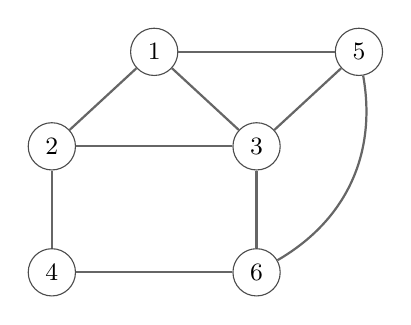
\begin{tikzpicture}[x=1cm,y=1cm]
\node[bt-gv] (g1) at (0,1.2) {1};
\node[bt-gv] (g2) at (-1.3,0) {2};
\node[bt-gv] (g3) at (1.3,0) {3};
\node[bt-gv] (g4) at (-1.3,-1.6) {4};
\node[bt-gv] (g5) at (2.6,1.2) {5};
\node[bt-gv] (g6) at (1.3,-1.6) {6};
\draw[bt-ge] (g1) -- (g2);
\draw[bt-ge] (g1) -- (g3);
\draw[bt-ge] (g1) -- (g5);
\draw[bt-ge] (g2) -- (g3);
\draw[bt-ge] (g2) -- (g4);
\draw[bt-ge] (g3) -- (g5);
\draw[bt-ge] (g3) -- (g6);
\draw[bt-ge] (g4) -- (g6);
\draw[bt-ge] (g5) to[bend left=35] (g6);
\end{tikzpicture}
\diagcaption{$m$ 著色的例子：$6$ 個頂點、$9$ 條邊。}
\label{fig:bk-graph}
\end{center}

\begin{center}
\begin{tabular}{cccll}
\toprule
步驟 & $k$ & $c$ & 部分解 $x_1 \ldots x_{k-1}$ & 結果 \\
\midrule
1 & 1 & 1 & （空） & 通過 \\
2 & 2 & 1 & 1 & 和頂點 1 同色 \\
3 & 2 & 2 & 1 & 通過 \\
4 & 3 & 1 & 1 2 & 和頂點 1 同色 \\
5 & 3 & 2 & 1 2 & 和頂點 2 同色 \\
6 & 3 & 3 & 1 2 & 通過 \\
7 & 4 & 1 & 1 2 3 & 通過 \\
8 & 5 & 1 & 1 2 3 1 & 和頂點 1 同色 \\
9 & 5 & 2 & 1 2 3 1 & 通過 \\
10 & 6 & 1 & 1 2 3 1 2 & 和頂點 4 同色 \\
11 & 6 & 2 & 1 2 3 1 2 & 和頂點 5 同色 \\
12 & 6 & 3 & 1 2 3 1 2 & 和頂點 3 同色；頂點 6 三色都不行，退回 \\
13 & 5 & 3 & 1 2 3 1 & 和頂點 3 同色；頂點 5 試完，退回 \\
14 & 4 & 2 & 1 2 3 & 和頂點 2 同色 \\
15 & 4 & 3 & 1 2 3 & 通過 \\
16 & 5 & 1 & 1 2 3 3 & 和頂點 1 同色 \\
17 & 5 & 2 & 1 2 3 3 & 通過 \\
18 & 6 & 1 & 1 2 3 3 2 & 通過，得到塗法 $(1, 2, 3, 3, 2, 1)$ \\
\bottomrule
\end{tabular}
\end{center}

連根一共產生 $19$ 個節點。 步驟 7 把頂點 4 塗成 $1$，當下沒有衝突，但頂點 6 同時和頂點 3
（色 $3$）、4（色 $1$）、5（色 $2$）相鄰，三種顏色都被占走。 回溯一路退到頂點 4，改塗
$3$ 之後才走得通。 這個錯誤要到兩層之後才看得出來，界限函數只檢查已經塗色的鄰居，沒辦法
提早發現。

搜尋完整棵樹會找到 $6$ 種塗法（連根產生 $121$ 個節點），它們其實是同一種分組換顏色名
字：$\{1, 6\}$、$\{2, 5\}$、$\{3, 4\}$ 三組，三種顏色排列有 $3! = 6$ 種。 只想知道「能不能
塗」或想數「本質上不同」的塗法時，可以固定頂點 1 塗顏色 $1$，節點數降到 $41$，找到的 $2$
種塗法乘上 $3$ 就是全部（固定一個頂點只消掉 $3$ 倍；要消掉全部 $3!$ 倍，得再規定顏色第一
次出現的順序）。 $n$ 皇后也能這樣去掉對稱：解左右翻轉還是解，第 1 列只要試前
$\lceil n / 2 \rceil$ 欄，找到的解再翻轉一次（$n$ 是奇數時，第 1 列放正中間的解翻轉後還
是第 1 列放正中間，不能直接乘 $2$）。

\section{分支限界}
\label{sec:bk-bb}

\subsection{E-節點怎麼選：FIFO、LIFO 與最小成本}

回溯一產生子節點就往下走，原來的 E-節點要等整棵子樹走完才繼續。 \textbf{分支限界}
（branch and bound）換一種做法：E-節點一次把所有子節點都產生出來，沒被剪掉的子節點成為活節
點，放進一個容器；然後從容器裡取出下一個 E-節點。 容器怎麼取，決定了搜尋的順序：

\begin{itemize}
\item \textbf{FIFO 分支限界}：容器是佇列，先放進去的先取出，節點依層的順序展開，和廣度優
先搜尋一樣。
\item \textbf{LIFO 分支限界}：容器是堆疊，最後放進去的先取出。 它也往深處走，但每個
E-節點先產生全部的子節點，和回溯的深度優先不完全相同，有的課本叫它 D-search。
\item \textbf{最小成本分支限界}（least-cost，LC）：每個活節點有一個估計值 $\hat c(x)$，代表
「經過 $x$ 的答案，成本大約是多少」，每次取 $\hat c$ 最小的；容器是第~8~章的優先佇列。 求
最大值時改成取上界最大的，這種做法也叫\textbf{最佳優先搜尋}（best-first search）。
\end{itemize}

\textbf{可行性剪枝與界限剪枝。} 第~\ref{sec:bk-tree}~節的界限函數都在回答同一個問題：這個
部分解還有沒有可能補成一個合法的解？ $n$ 皇后檢查對角線、子集合和檢查會不會超過或湊不
到、著色檢查鄰居的顏色，都是這一類，叫做\textbf{可行性剪枝}（feasibility pruning）。 分支
限界通常用來解\textbf{最佳化問題}（要找最大或最小的解），這時還有第二種剪枝：搜尋時記住
目前找到的最好的解，如果能對一個節點算出一個\textbf{界限}，保證這棵子樹裡每一個解都不會比
目前最好的解更好，整棵子樹就可以丟掉，叫做\textbf{界限剪枝}（bounding）。 求最大值時用
\textbf{上界}，求最小值時用\textbf{下界}。 章首的兩種「不必再試」正好是這兩種：超重是可行
性剪枝，「剩下的全部都拿也比不上已經找到的組合」是界限剪枝。

界限要「樂觀」：求最大值的上界寧可估得太大，不能估得太小。 估得太小會把真正的最佳解剪
掉，答案就錯了；估得太大只是剪得少、跑得慢。 在不估錯的前提下，越接近真實值的界限剪得越
多，但通常也算得越久。

界限在分支限界裡有兩個用途：決定先展開哪個節點（只有 LC 用到），以及剪掉不可能比目前最好
的解更好的節點（三種都用）。 以求最小值為例，令 $\mathit{upper}$ 是目前找到的最好答案的
成本，$\hat c(x)$ 是 $x$ 子樹裡所有答案成本的下界；$\hat c(x) \ge \mathit{upper}$ 的節點不必
再展開。

\begin{pseudo}[label=alg:bk-lc]{最小成本分支限界（求最小值）}
\Function{LC-Search}{}
    \State $\mathit{upper} \gets \infty$；把根放進活節點集合 $L$
    \While{$L$ 不是空的}
        \State $E \gets L$ 裡 $\hat c$ 最小的節點（一樣小時取編號小的），從 $L$ 移除
        \If{$\hat c(E) \ge \mathit{upper}$}
            \State \Return $\mathit{upper}$ \Comment{剩下的節點都不可能更好}
        \EndIf
        \For{$E$ 的每一個子節點 $X$，依固定的順序產生並編號}
            \State 算出 $\hat c(X)$
            \If{$X$ 是答案節點}
                \If{$\hat c(X) < \mathit{upper}$}
                    \State $\mathit{upper} \gets \hat c(X)$，記下 $X$
                \EndIf
            \ElsIf{$\hat c(X) < \mathit{upper}$}
                \State 把 $X$ 放進 $L$
            \EndIf
        \EndFor
    \EndWhile
    \State \Return $\mathit{upper}$
\EndFunction
\end{pseudo}

第 4 行改成「取最早放進 $L$ 的節點」就是 FIFO，改成「取最晚放進 $L$ 的節點」就是 LIFO，
其他行都不變。 這個程序要正確，$\hat c$ 必須滿足兩件事：對每個節點，$\hat c(x)$ 不超過
$x$ 子樹裡任何答案的真正成本；在答案節點上，$\hat c$ 就是真正的成本。 這樣第 5 行取出的
節點 $\hat c$ 已經不小於 $\mathit{upper}$ 時，$L$ 裡每個節點的 $\hat c$ 都不小於
$\mathit{upper}$，它們的子樹裡不會有更便宜的答案，$\mathit{upper}$ 就是最佳解的成本。

\subsection{0/1 背包的最佳優先分支限界}
\label{sec:bk-knap}

$n$ 個物品，第 $i$ 個價值 $p_i$、重量 $w_i$，背包容量 $W$，要選一些物品使總重不超過 $W$、
總價值最大。 第~18、19~章把價值寫成 $v_i$；這一章照分支限界課本的習慣寫成 $p_i$（profit），
因為 $v$ 要留給樹上的節點。 狀態空間樹和子集合和一樣是滿二元樹，第 $k$ 層決定第 $k$ 個物品
拿或不拿。 每一個節點本身就是一個合法的解（後面的物品都不拿），所以只要沒超重，就可以拿
它的總價值去更新目前最好的值 $\mathit{best}$。

背包求最大值，要的是上界。 最省事的上界是「目前的總價值加上剩下所有物品的價值」，完全不
管容量，很鬆。 好得多的做法是把剩下的物品當成可以切開：先把物品依 $p_i / w_i$ 由大到小排
好，放得下就整個放，放不下就放進剛好填滿的那一部分。 這就是第~19~章分數背包的貪心解
（虛擬碼~\ref{alg:gr-frac}），加上目前的總價值 $P$ 當作上界：

\begin{pseudo}[label=alg:bk-bound, unbreakable]{分數背包上界}
\Function{Bound}{$k, P, \mathit{Wt}$} \Comment{已決定前 $k$ 個物品，$\mathit{Wt} \le W$}
    \State $b \gets P$；$\mathit{room} \gets W - \mathit{Wt}$；$i \gets k + 1$
    \While{$i \le n$ \AND $w_i \le \mathit{room}$}
        \State $\mathit{room} \gets \mathit{room} - w_i$；$b \gets b + p_i$；$i \gets i + 1$
    \EndWhile
    \If{$i \le n$}
        \State $b \gets b + p_i \cdot \mathit{room} / w_i$ \Comment{第 $i$ 個只放一部分}
    \EndIf
    \State \Return $b$
\EndFunction
\end{pseudo}

這個上界不會估得太小。 這棵子樹裡的任何一個解，都是在剩下的物品 $k + 1, \ldots, n$ 裡選一
個總重不超過 $\mathit{room} = W - \mathit{Wt}$ 的子集合 $T$，總價值是 $P + \sum_{i \in T} p_i$。
把 $T$ 看成「每個物品只拿 $0$ 或 $1$ 份」，它也是同一組物品、同一個容量下分數背包的一個
解；定理~\ref{thm:gr-frac} 說貪心解是分數背包的最佳解，所以 \proc{Bound} 回傳的值不小於
$P + \sum_{i \in T} p_i$。 每次算 \proc{Bound} 要 $O(n)$ 的時間，但它比「剩下的全拿」緊得
多，剪掉的節點也多得多。

分支限界每次展開上界最大的活節點（最佳優先）。 規則整理如下：

\begin{enumerate}
\item 物品依 $p_i / w_i$ 由大到小排好；$\mathit{best} \gets 0$（什麼都不拿也是一個解）。
\item 每個節點記錄層數 $k$（前 $k$ 個物品已決定）、總價值 $P$、總重 $\mathit{Wt}$ 和上界
$b$。 根是節點 1。
\item 從活節點裡取出 $b$ 最大的（一樣大時取編號小的）。 如果 $b \le \mathit{best}$，它是在放
進來之後才變得沒希望的，直接丟掉；否則它是 E-節點。
\item E-節點先產生「拿第 $k + 1$ 個物品」的子節點，再產生「不拿」的子節點，依序編號。 超重的子
節點直接死掉；沒超重的子節點先用 $P$ 更新 $\mathit{best}$，再算 $b$，$k + 1 < n$ 而且 $b >
\mathit{best}$ 才放進活節點。
\end{enumerate}

\begin{pseudo}[label=alg:bk-knap-bb]{0/1 背包的最佳優先分支限界}
\Function{Knapsack-BB}{}
    \State 物品依 $p_i / w_i$ 由大到小排好；$\mathit{best} \gets 0$
    \State 根 $\gets (k = 0, P = 0, \mathit{Wt} = 0)$，$\mathit{root}.b \gets \Call{Bound}{0, 0, 0}$，放進優先佇列 $Q$
    \While{$Q$ 不是空的}
        \State $v \gets Q$ 裡 $b$ 最大的節點（一樣大時取編號小的），從 $Q$ 移除
        \If{$v.b > \mathit{best}$} \Comment{否則 $v$ 已經沒希望，丟掉}
            \For{先「拿」再「不拿」第 $v.k + 1$ 個物品}
                \State 產生子節點 $u$，算出 $u.k$、$u.P$、$u.\mathit{Wt}$，並編號
                \If{$u.\mathit{Wt} \le W$} \Comment{超重的子節點直接死掉}
                    \If{$u.P > \mathit{best}$}
                        \State $\mathit{best} \gets u.P$，記下 $u$ 拿了哪些物品
                    \EndIf
                    \State $u.b \gets \Call{Bound}{u.k, u.P, u.\mathit{Wt}}$
                    \If{$u.k < n$ \AND $u.b > \mathit{best}$}
                        \State 把 $u$ 放進 $Q$
                    \EndIf
                \EndIf
            \EndFor
        \EndIf
    \EndWhile
    \State \Return $\mathit{best}$
\EndFunction
\end{pseudo}

\subsubsection{手算追蹤}

背包容量 $W = 13$，四個物品已經依價值密度排好：

\begin{center}
\begin{tabular}{ccccc}
\toprule
物品 & 1 & 2 & 3 & 4 \\
\midrule
價值 $p_i$ & 27 & 12 & 20 & 15 \\
重量 $w_i$ & 3 & 2 & 4 & 5 \\
$p_i / w_i$ & 9 & 6 & 5 & 3 \\
\bottomrule
\end{tabular}
\end{center}

根的上界：物品 1、2、3 整個放進去，價值 $59$、重量 $9$，剩下的容量 $4$ 放物品 4 的
$4/5$，價值 $15 \cdot 4/5 = 12$，上界 $71$。 下表每一列是一個 E-節點產生的兩個子節點，「之後的
$Q$」列出這一步做完時佇列裡的節點和它們的上界。

\begin{center}
\small
\begin{tabular}{clccccl}
\toprule
E-節點 & 子節點 & $P$ & $\mathit{Wt}$ & $b$ & $\mathit{best}$ & 結果 \\
\midrule
1 & 2：拿 1 & 27 & 3 & 71 & 27 & 活 \\
 & 3：不拿 1 & 0 & 0 & 47 & 27 & 活；$Q$：2(71)、3(47) \\
\midrule
2 & 4：拿 2 & 39 & 5 & 71 & 39 & 活 \\
 & 5：不拿 2 & 27 & 3 & 62 & 39 & 活；$Q$：4(71)、5(62)、3(47) \\
\midrule
4 & 6：拿 3 & 59 & 9 & 71 & 59 & 活 \\
 & 7：不拿 3 & 39 & 5 & 54 & 59 & 死（$54 \le 59$）；$Q$：6(71)、5(62)、3(47) \\
\midrule
6 & 8：拿 4 & 74 & 14 & -- & 59 & 超重 \\
 & 9：不拿 4 & 59 & 9 & 59 & 59 & 死（最後一層）；$Q$：5(62)、3(47) \\
\midrule
5 & 10：拿 3 & 47 & 7 & 62 & 59 & 活 \\
 & 11：不拿 3 & 27 & 3 & 42 & 59 & 死；$Q$：10(62)、3(47) \\
\midrule
10 & 12：拿 4 & 62 & 12 & 62 & 62 & 新的 $\mathit{best}$，最後一層；$Q$：3(47) \\
 & 13：不拿 4 & 47 & 7 & 47 & 62 & 死 \\
\midrule
3 & \multicolumn{6}{l}{取出時 $47 \le 62$，丟掉；$Q$ 空了，結束} \\
\bottomrule
\end{tabular}
\end{center}

\begin{center}
\begin{tikzpicture}[x=1.3cm,y=1.05cm]
\node[bt-kexp, label={[bt-num]left:1}, label={[bt-ord]above right:1}] (k1) at (7.0,0.0) {0,0\\[-1pt]71};
\node[bt-kexp, label={[bt-num]left:2}, label={[bt-ord]above right:2}] (k2) at (4.4,-1.4) {27,3\\[-1pt]71};
\node[bt-kdead, label={[bt-num]left:3}] (k3) at (9.6,-1.4) {0,0\\[-1pt]47};
\node[bt-kexp, label={[bt-num]left:4}, label={[bt-ord]above right:3}] (k4) at (2.0,-2.8) {39,5\\[-1pt]71};
\node[bt-kexp, label={[bt-num]left:5}, label={[bt-ord]above right:5}] (k5) at (6.8,-2.8) {27,3\\[-1pt]62};
\node[bt-kexp, label={[bt-num]left:6}, label={[bt-ord]above right:4}] (k6) at (0.8,-4.2) {59,9\\[-1pt]71};
\node[bt-kdead, label={[bt-num]left:7}] (k7) at (3.2,-4.2) {39,5\\[-1pt]54};
\node[bt-kdead, label={[bt-num]left:8}] (k8) at (0.0,-5.6) {74,14\\[-1pt]$\times$};
\node[bt-kdead, label={[bt-num]left:9}] (k9) at (1.6,-5.6) {59,9\\[-1pt]59};
\node[bt-kexp, label={[bt-num]left:10}, label={[bt-ord]above right:6}] (k10) at (5.6,-4.2) {47,7\\[-1pt]62};
\node[bt-kdead, label={[bt-num]left:11}] (k11) at (8.0,-4.2) {27,3\\[-1pt]42};
\node[bt-kbest, label={[bt-num]left:12}] (k12) at (4.8,-5.6) {62,12\\[-1pt]62};
\node[bt-kdead, label={[bt-num]left:13}] (k13) at (6.4,-5.6) {47,7\\[-1pt]47};
\draw[bt-e] (k1) -- node[bt-el] {1} (k2);
\draw[bt-e] (k1) -- node[bt-el] {0} (k3);
\draw[bt-e] (k2) -- node[bt-el] {1} (k4);
\draw[bt-e] (k2) -- node[bt-el] {0} (k5);
\draw[bt-e] (k4) -- node[bt-el] {1} (k6);
\draw[bt-e] (k4) -- node[bt-el] {0} (k7);
\draw[bt-e] (k6) -- node[bt-el] {1} (k8);
\draw[bt-e] (k6) -- node[bt-el] {0} (k9);
\draw[bt-e] (k5) -- node[bt-el] {1} (k10);
\draw[bt-e] (k5) -- node[bt-el] {0} (k11);
\draw[bt-e] (k10) -- node[bt-el] {1} (k12);
\draw[bt-e] (k10) -- node[bt-el] {0} (k13);
\end{tikzpicture}
\diagcaption{0/1 背包的最佳優先分支限界。 方框上一行是 $P, \mathit{Wt}$，下一行是上界
$b$；左邊的小字是產生的順序，藍色框右上角的粗體數字是它被選為 E-節點的順序。 邊上的 $1$、$0$
表示拿或不拿。 虛線是死節點，橘色是最後的最佳解。}
\label{fig:bk-knap}
\end{center}

這個過程有三個地方要看清楚。 第一，節點 5 比節點 6 早產生，卻比較晚展開：節點 6 的上界 $71$ 比
節點 5 的 $62$ 大，最佳優先搜尋不管節點在哪一層，只看上界。 第二，節點 9 的 $P = 59$ 等於
當時的 $\mathit{best}$，它已經是最後一層，不必放進佇列。 第三，節點 3 在第一步就放進佇
列，上界 $47$ 當時大於 $\mathit{best} = 27$；等到它被取出時 $\mathit{best}$ 已經是 $62$，
才在第 6 行被丟掉。 最佳解是物品 1、3、4，總重 $12$，總價值 $62$，一共產生 $13$ 個節點；整
棵狀態空間樹（滿二元樹）有 $2^5 - 1 = 31$ 個節點。 用第~18~章的動態規劃算這組資料，答案也是 $62$。

\begin{examnote}
背包的分支限界題，先檢查物品有沒有依 $p_i / w_i$ 由大到小排好，沒有的話先排，並寫出排序後
的編號。 本書的約定：先產生「拿」再產生「不拿」；超重的子節點也編號；上界一樣時取編號小
的；$b \le \mathit{best}$ 就剪（等於也剪，因為不可能更好）。 每個節點寫出 $P$、$\mathit{Wt}$、
$b$，並另外列出 E-節點的順序和 $\mathit{best}$ 的變化。 有些課本把背包改寫成求最小值（價值
取負號），每個節點同時算一個下界 $\hat c$ 和一個用貪心整數解得到的上界 $u$，用 $u$ 來更新
$\mathit{upper}$；樹的形狀一樣，但節點被剪掉的時機可能不同，題目指定哪一種就照哪一種寫。
\end{examnote}

\subsubsection{三種順序的比較}

把第 5 行改成 FIFO 或 LIFO，其他規則不變（子節點一樣先拿後不拿，LIFO 因此先展開「不拿」的子
節點），產生的節點數如下。 第二組資料有 $20$ 個物品，第 $i$ 個的重量是
$10 + (37 i \bmod 41)$，價值是重量加上 $(53 i \bmod 29) + 5$，容量取總重的一半 $295$；物品先
依 $p_i / w_i$ 由大到小重新排過，最佳解是 $586$。

\begin{center}
\begin{tabular}{lcccc}
\toprule
 & \multicolumn{2}{c}{4 個物品} & \multicolumn{2}{c}{20 個物品} \\
順序 & 產生的節點 & E-節點 & 產生的節點 & E-節點 \\
\midrule
FIFO & 15 & 7 & 2283 & 1141 \\
LIFO & 23 & 11 & 6175 & 3087 \\
最佳優先 & 13 & 6 & 37 & 18 \\
\bottomrule
\end{tabular}
\end{center}

FIFO 一層一層展開，要到很深的地方才找到好的 $\mathit{best}$，前面幾層的節點很多都剪不掉；
LIFO 在這裡先往「不拿」的方向衝，找到的 $\mathit{best}$ 很差，剪得更少。 最佳優先第一條走
的就是貪心的方向，$\mathit{best}$ 很快就接近最佳解。 代價是記憶體：最佳優先搜尋要把所有活
節點留在佇列裡，最壞情況和節點數同一個量級；回溯只需要一條從根到目前節點的路徑。

\subsubsection{C 程式}

活節點放在一個用 \texttt{realloc} 加倍的陣列裡，每次掃過一遍挑出上界最大的（一樣大時取編號
小的），挑出來的位置用最後一個節點補上。 每次挑選要 $O(\ell)$，$\ell$ 是當時的活節點數；活節點多的時
候改用第~8~章的堆積，挑選就只要 $O(\lg \ell)$。 每個節點用一個 \texttt{unsigned long} 的位元記錄拿了
哪些物品，不必另外存父節點。 輸入的物品要先依 $p_i / w_i$ 由大到小排好；物品資料讀入後不再
改，放在檔案範圍的陣列。 程式印出每一個 E-節點的 $P$、$\mathit{Wt}$、$b$，以及最後被丟掉的節點。

\begin{example}[label=ex:bk-knapsack-bb]{c}{(knapsack\_bb.c) 0/1 背包的最佳優先分支限界}
#include <stdio.h>
#include <stdlib.h>

typedef struct {
    int id, level, profit, weight;  // 編號、已決定幾個、價值、重量
    double bound;                   // 子樹的價值上界
    unsigned long take;             // 第 i 個位元：拿了第 i 個物品
} Node;

// 活節點放在一個可以變長的陣列裡；每次掃過一遍挑出上界最大的
typedef struct {
    Node *a;
    int size, cap;
} List;

static int add(List *q, Node v)
{
    if (q->size == q->cap) {
        int cap = q->cap ? 2 * q->cap : 16;
        Node *a = realloc(q->a, cap * sizeof *a);
        if (a == NULL) {
            return 0;
        }
        q->a = a;
        q->cap = cap;
    }
    q->a[q->size++] = v;
    return 1;
}

// 取出上界最大的節點；上界一樣大時取編號小的
static Node take_best(List *q)
{
    int b = 0;
    for (int i = 1; i < q->size; i++) {
        Node *x = &q->a[i], *y = &q->a[b];
        if (x->bound > y->bound
            || (x->bound == y->bound && x->id < y->id)) {
            b = i;
        }
    }
    Node v = q->a[b];
    q->a[b] = q->a[--q->size];      // 拿最後一個補洞
    return v;
}

static int n, cap, p[30], w[30];    // 物品已依 p/w 由大到小排好

// 分數背包上界
static double bound(int level, int profit, int weight)
{
    double b = profit;
    int room = cap - weight;
    for (int i = level; i < n; i++) {
        if (w[i] > room) {
            return b + (double)(p[i] * room) / w[i];
        }
        room -= w[i];
        b += p[i];
    }
    return b;
}

int main(void)
{
    if (scanf("%d %d", &n, &cap) != 2 || n < 1 || n > 30) {
        return 1;
    }
    for (int i = 0; i < n; i++) {
        if (scanf("%d %d", &p[i], &w[i]) != 2 || w[i] <= 0) {
            return 1;
        }
    }
    List q = {NULL, 0, 0};
    int count = 1, best = 0;
    unsigned long best_take = 0;
    int ok = add(&q, (Node){1, 0, 0, 0, bound(0, 0, 0), 0});
    while (ok && q.size > 0) {
        Node v = take_best(&q);
        if (v.bound <= best) {
            printf("drop %d: b=%g\n", v.id, v.bound);
            continue;
        }
        printf("expand %d: P=%d Wt=%d b=%g\n",
               v.id, v.profit, v.weight, v.bound);
        for (int t = 1; t >= 0 && ok; t--) {    // 先拿，再不拿
            int k = v.level;
            Node u = {++count, k + 1, v.profit + t * p[k],
                      v.weight + t * w[k], 0,
                      v.take | (unsigned long)t << k};
            if (u.weight > cap) {
                continue;                               // 超重
            }
            if (u.profit > best) {
                best = u.profit;
                best_take = u.take;
            }
            u.bound = bound(u.level, u.profit, u.weight);
            if (u.level < n && u.bound > best) {
                ok = add(&q, u);
            }
        }
    }
    printf("best %d, items:", best);
    for (int i = 0; i < n; i++) {
        if (best_take >> i & 1) {
            printf(" %d", i + 1);
        }
    }
    printf("\nnodes generated: %d\n", count);
    free(q.a);
    return ok ? 0 : 1;
}
\end{example}
\iosample{4 13 \\ 27 3 \\ 12 2 \\ 20 4 \\ 15 5}{expand 1: P=0 Wt=0 b=71 \\ expand 2: P=27 Wt=3 b=71 \\ expand 4: P=39 Wt=5 b=71 \\ expand 6: P=59 Wt=9 b=71 \\ expand 5: P=27 Wt=3 b=62 \\ expand 10: P=47 Wt=7 b=62 \\ drop 3: b=47 \\ best 62, items: 1 3 4 \\ nodes generated: 13}

E-節點的順序 1、2、4、6、5、10 和手算表一樣。 上界是 \texttt{double}，用 \texttt{\%g} 印，
整數就印成整數。 \texttt{bound} 裡 \texttt{p * room} 先用整數乘好再除，真正的上界是整數時算出
來的 \texttt{double} 也剛好是那個整數，和整數 \texttt{best} 比較不會因為誤差而判斷錯。

\subsection{旅行推銷員問題：縮減矩陣}
\label{sec:bk-tsp}

\textbf{旅行推銷員問題}（traveling salesperson problem，TSP）：有 $n$ 個城市，$C[i][j]$ 是從
城市 $i$ 到城市 $j$ 的成本（$C[i][j]$ 和 $C[j][i]$ 可以不同），要從城市 1 出發，每個城市恰好
經過一次，最後回到城市 1，總成本最小。 這樣的路線有 $(n - 1)!$ 條。 第~28~章會說明這個問
題是 NP 難的，目前沒有已知的多項式時間演算法；分支限界可以讓小規模的實例不必列舉全部路
線。

狀態空間樹的根是只含城市 1 的路徑；一個節點代表一條從 1 出發的路徑，它的子節點是在路徑後面
接上一個還沒去過的城市，依城市編號由小到大產生。 深度 $n - 1$ 的葉節點已經走過所有城市，接
上回到 1 的邊就是一條完整的路線。 $n = 5$ 時這棵樹有 $1 + 4 + 12 + 24 + 24 = 65$ 個節點。

\subsubsection{縮減矩陣與下界}

把成本矩陣的對角線設成 $\infty$（不能從一個城市走到自己）。 一條路線從每個城市恰好出發
一次、也恰好進入每個城市一次，所以它在矩陣的每一列恰好用到一格，每一行也恰好用到一格。
於是把某一列的每一格都減去同一個數 $m$，每一條路線的成本都恰好少 $m$，誰比較便宜不會
改變。

\textbf{縮減}（reduce）一個矩陣：先對每一列，減去該列的最小值；再對每一行，減去該行（列
縮減之後）的最小值。 全部是 $\infty$ 的列或行不動。 縮減後每一列、每一行都至少有一個
$0$，所有的格子都不是負數。 減掉的總量叫做\textbf{縮減量} $r$。 任何一條路線，原來的成本
等於 $r$ 加上它在縮減後矩陣上的成本，後者不小於 $0$，所以 $r$ 是每一條路線成本的下界，
也就是根的 $\hat c$。

\begin{pseudo}[label=alg:bk-reduce]{縮減矩陣}
\Function{Reduce}{$A$} \Comment{就地修改 $A$；$\infty - m = \infty$}
    \State $r \gets 0$
    \For{$i \gets 1$ \To $n$}
        \State $m \gets$ 第 $i$ 列的最小值
        \If{$0 < m < \infty$}
            \State 第 $i$ 列的每一格減去 $m$；$r \gets r + m$
        \EndIf
    \EndFor
    \For{$j \gets 1$ \To $n$}
        \State $m \gets$ 第 $j$ 行的最小值
        \If{$0 < m < \infty$}
            \State 第 $j$ 行的每一格減去 $m$；$r \gets r + m$
        \EndIf
    \EndFor
    \State \Return $r$
\EndFunction
\end{pseudo}

\textbf{子節點的下界。} 設節點 $S$ 的路徑停在城市 $i$，它的縮減矩陣是 $A$，下界是 $\hat c(S)$。
接上城市 $j$ 得到子節點 $T$：

\begin{pseudo}[label=alg:bk-tsp-child]{TSP 的子節點}
\Function{TSP-Child}{$A, \hat c(S), i, j$}
    \State $B \gets A$ 的複本
    \State $B$ 的第 $i$ 列、第 $j$ 行每一格都設成 $\infty$ \Comment{$i$ 的出邊、$j$ 的入邊已經決定}
    \State $B[j][1] \gets \infty$ \Comment{不能還沒走完就回到 1}
    \State $r \gets \Call{Reduce}{B}$
    \State \Return $B$ 和 $\hat c(T) = \hat c(S) + A[i][j] + r$
\EndFunction
\end{pseudo}

第 3 行：路線已經決定從 $i$ 走到 $j$，$i$ 不會再從別的邊出發，$j$ 也不會再從別的邊進入。
第 4 行：路徑 $1 \to \cdots \to j$ 如果接著走 $j \to 1$，會在還沒經過所有城市時就繞回起點。
$\hat c(T)$ 由三部分組成：父節點已經算進來的下界、這條邊在父節點矩陣上剩下的成本
$A[i][j]$、以及新矩陣再縮減一次的量 $r$。

\begin{whybox}[縮減矩陣給出的是下界，葉節點上剛好是路線成本]
設 $n \ge 3$。 對每個不是葉節點的節點 $X$（路徑 $P_X$ 停在城市 $i$，縮減矩陣 $A_X$），下面的
等式對每一條以 $P_X$ 開頭的路線 $T$ 都成立：
\[
\text{$T$ 的成本} = \hat c(X) + \sum_{e \in T \setminus P_X} A_X[e]. \tag{$*$}
\]
$A_X$ 的每一格都不是負數，所以 $\hat c(X)$ 不超過 $T$ 的成本。

根：路線在每一列、每一行各用一格，縮減時每減掉一個 $m$，每條路線的成本都少 $m$，($*$)
成立。 從 $X$ 到子節點 $Y$（接上 $j$）：以 $P_Y$ 開頭的路線一定用 $(i, j)$，它剩下的邊
$T \setminus P_Y$ 從 $j$ 和還沒去過的城市各出發一次，進入還沒去過的城市和城市 1 各一
次。 第 3、4 行設成 $\infty$ 的格子，這些邊都用不到（$Y$ 不是葉節點時，還有城市沒去，$j \to
1$ 不會出現在 $T$ 裡）。 $B$ 裡還有有限值的列和行，恰好是這些邊用到的列和行，各用一格，
所以縮減掉的 $r$ 對每一條這樣的路線都恰好少算一次，($*$) 對 $Y$ 也成立。

葉節點：設葉節點的父節點 $X$ 的路徑停在 $i$，只剩城市 $j$ 沒去。 $A_X$ 第 $j$ 列除了 $A_X[j][1]$
以外都是 $\infty$，縮減後這一格一定是 $0$；又 $A_X[i][1] = \infty$，所以 $X$ 的路線只有
$i \to j \to 1$ 這一條，($*$) 給出它的成本是 $\hat c(X) + A_X[i][j] + 0$。 葉節點的 $B$ 全部是
$\infty$，$r = 0$，$\hat c(\text{葉節點}) = \hat c(X) + A_X[i][j]$，正好等於這條路線的成本。
\end{whybox}

\subsubsection{手算追蹤：5 個城市}

成本矩陣如下（列是出發的城市，行是到達的城市）。 先做列縮減：五列的最小值是 $4$、$10$、
$3$、$10$、$9$，共 $36$。 減完之後，第 1、2、3 行已經有 $0$，第 4 行的最小值是 $8$，第 5 行
是 $6$，共 $14$。 根的下界 $\hat c = 36 + 14 = 50$，縮減後的矩陣是節點 1 的矩陣。

\begin{center}
\footnotesize
\setlength{\tabcolsep}{4pt}
\begin{tabular}[t]{c|ccccc}
\multicolumn{6}{c}{原始成本矩陣}\\
 & 1 & 2 & 3 & 4 & 5 \\\hline
1 & $\infty$ & 7 & 4 & 21 & 16 \\
2 & 20 & $\infty$ & 10 & 20 & 16 \\
3 & 11 & 3 & $\infty$ & 11 & 16 \\
4 & 10 & 24 & 13 & $\infty$ & 25 \\
5 & 9 & 16 & 24 & 24 & $\infty$ \\
\end{tabular}\qquad
\begin{tabular}[t]{c|ccccc}
\multicolumn{6}{c}{縮減後＝節點 1（$\hat c = 50$）}\\
 & 1 & 2 & 3 & 4 & 5 \\\hline
1 & $\infty$ & 3 & 0 & 9 & 6 \\
2 & 10 & $\infty$ & 0 & 2 & 0 \\
3 & 8 & 0 & $\infty$ & 0 & 7 \\
4 & 0 & 14 & 3 & $\infty$ & 9 \\
5 & 0 & 7 & 15 & 7 & $\infty$ \\
\end{tabular}
\end{center}

LC 搜尋的過程如下。 每一步從活節點裡取 $\hat c$ 最小的當 E-節點，產生它所有的子節點。 下表
列出每一個產生的子節點：$A[i][j]$ 是父節點矩陣上那一格，「再縮減」寫出子節點的矩陣減了哪幾
列、哪幾行。

\begin{center}
\small
\begin{tabular}{cclcclcc}
\toprule
節點 & 父 & 路徑 & $\hat c(\text{父})$ & $A[i][j]$ & 再縮減 & $r$ & $\hat c$ \\
\midrule
2 & 1 & 1$\to$2 & 50 & 3 & 不用減 & 0 & 53 \\
3 & 1 & 1$\to$3 & 50 & 0 & 不用減 & 0 & 50 \\
4 & 1 & 1$\to$4 & 50 & 9 & 列 4 減 3 & 3 & 62 \\
5 & 1 & 1$\to$5 & 50 & 6 & 列 5 減 7 & 7 & 63 \\
\midrule
6 & 3 & 1$\to$3$\to$2 & 50 & 0 & 行 4 減 2 & 2 & 52 \\
7 & 3 & 1$\to$3$\to$4 & 50 & 0 & 列 4 減 9、行 2 減 5 & 14 & 64 \\
8 & 3 & 1$\to$3$\to$5 & 50 & 7 & 列 2 減 2、列 5 減 7 & 9 & 66 \\
\midrule
9 & 6 & 1$\to$3$\to$2$\to$4 & 52 & 0 & 列 4 減 9 & 9 & 61 \\
10 & 6 & 1$\to$3$\to$2$\to$5 & 52 & 0 & 列 5 減 5 & 5 & 57 \\
\midrule
11 & 2 & 1$\to$2$\to$3 & 53 & 0 & 行 5 減 7 & 7 & 60 \\
12 & 2 & 1$\to$2$\to$4 & 53 & 2 & 列 3 減 7、列 4 減 3 & 10 & 65 \\
13 & 2 & 1$\to$2$\to$5 & 53 & 0 & 列 5 減 7、行 3 減 3 & 10 & 63 \\
\midrule
14 & 10 & 1$\to$3$\to$2$\to$5$\to$4 & 57 & 0 & 不用減（葉節點） & 0 & 57 \\
\bottomrule
\end{tabular}
\end{center}

E-節點依序是節點 1（$50$）、3（$50$）、6（$52$）、2（$53$）、10（$57$）。 展開節點 6 之後，活節
點裡最小的是節點 2 的 $53$，比節點 6 的子節點 10（$57$）小，搜尋跳回第 1 層。 節點 2 的三個子
節點都在 $60$ 以上，接著展開節點 10：它唯一的子節點 14 是葉節點，路線
$1 \to 3 \to 2 \to 5 \to 4 \to 1$ 的成本 $4 + 3 + 16 + 24 + 10 = 57$，$\mathit{upper} \gets 57$。 下
一個 $\hat c$ 最小的活節點是 11（$60$），$60 \ge 57$，停止。

最佳路線是 $1 \to 3 \to 2 \to 5 \to 4 \to 1$，成本 $57$。 一共產生 $14$ 個節點、展開 $5$ 個；
把 $24$ 條路線全部算一遍，最小值也是 $57$。 圖~\ref{fig:bk-tsp} 是整個過程的樹，
圖~\ref{fig:bk-tsp-mats} 是被展開的五個節點的縮減矩陣，算子節點的 $A[i][j]$ 和 $r$ 都從這
些矩陣來。

\begin{center}
\begin{tikzpicture}[x=1.4cm,y=1cm]
\node[bt-texp, label={[bt-cost]right:50}, label={[bt-ord]above right:1}] (t1) at (5.175,0.0) {1};
\node[bt-texp, label={[bt-cost]right:53}, label={[bt-ord]above right:4}] (t2) at (1.15,-1.25) {2};
\node[bt-texp, label={[bt-cost]right:50}, label={[bt-ord]above right:2}] (t3) at (5.462,-1.25) {3};
\node[bt-n, label={[bt-cost]right:62}] (t4) at (8.05,-1.25) {4};
\node[bt-n, label={[bt-cost]right:63}] (t5) at (9.2,-1.25) {5};
\node[bt-texp, label={[bt-cost]right:52}, label={[bt-ord]above right:3}] (t6) at (4.025,-2.5) {6};
\node[bt-n, label={[bt-cost]right:64}] (t7) at (5.75,-2.5) {7};
\node[bt-n, label={[bt-cost]right:66}] (t8) at (6.9,-2.5) {8};
\node[bt-n, label={[bt-cost]right:61}] (t9) at (3.45,-3.75) {9};
\node[bt-texp, label={[bt-cost]right:57}, label={[bt-ord]above right:5}] (t10) at (4.6,-3.75) {10};
\node[bt-n, label={[bt-cost]right:60}] (t11) at (0.0,-2.5) {11};
\node[bt-n, label={[bt-cost]right:65}] (t12) at (1.15,-2.5) {12};
\node[bt-n, label={[bt-cost]right:63}] (t13) at (2.3,-2.5) {13};
\node[bt-ans, label={[bt-cost]right:57}] (t14) at (4.6,-5.0) {14};
\draw[bt-e] (t1) -- node[bt-el] {2} (t2);
\draw[bt-e] (t1) -- node[bt-el] {3} (t3);
\draw[bt-e] (t1) -- node[bt-el] {4} (t4);
\draw[bt-e] (t1) -- node[bt-el] {5} (t5);
\draw[bt-e] (t3) -- node[bt-el] {2} (t6);
\draw[bt-e] (t3) -- node[bt-el] {4} (t7);
\draw[bt-e] (t3) -- node[bt-el] {5} (t8);
\draw[bt-e] (t6) -- node[bt-el] {4} (t9);
\draw[bt-e] (t6) -- node[bt-el] {5} (t10);
\draw[bt-e] (t2) -- node[bt-el] {3} (t11);
\draw[bt-e] (t2) -- node[bt-el] {4} (t12);
\draw[bt-e] (t2) -- node[bt-el] {5} (t13);
\draw[bt-e] (t10) -- node[bt-el] {4} (t14);
\end{tikzpicture}
\diagcaption{5 個城市的 LC 分支限界。 節點內是產生的順序，右邊是 $\hat c$，邊上是接上的城
市。 藍色是被展開的節點，右上角的粗體數字是展開的順序；橘色是找到的路線。}
\label{fig:bk-tsp}
\end{center}

\begin{center}
\footnotesize
\setlength{\tabcolsep}{3.5pt}
\begin{tabular}[t]{c|ccccc}
\multicolumn{6}{c}{節點 3（$\hat c = 50$）}\\
 & 1 & 2 & 3 & 4 & 5 \\\hline
1 & $\infty$ & $\infty$ & $\infty$ & $\infty$ & $\infty$ \\
2 & 10 & $\infty$ & $\infty$ & 2 & 0 \\
3 & $\infty$ & 0 & $\infty$ & 0 & 7 \\
4 & 0 & 14 & $\infty$ & $\infty$ & 9 \\
5 & 0 & 7 & $\infty$ & 7 & $\infty$ \\
\end{tabular}\qquad
\begin{tabular}[t]{c|ccccc}
\multicolumn{6}{c}{節點 6（$\hat c = 52$）}\\
 & 1 & 2 & 3 & 4 & 5 \\\hline
1 & $\infty$ & $\infty$ & $\infty$ & $\infty$ & $\infty$ \\
2 & $\infty$ & $\infty$ & $\infty$ & 0 & 0 \\
3 & $\infty$ & $\infty$ & $\infty$ & $\infty$ & $\infty$ \\
4 & 0 & $\infty$ & $\infty$ & $\infty$ & 9 \\
5 & 0 & $\infty$ & $\infty$ & 5 & $\infty$ \\
\end{tabular}

\medskip
\begin{tabular}[t]{c|ccccc}
\multicolumn{6}{c}{節點 2（$\hat c = 53$）}\\
 & 1 & 2 & 3 & 4 & 5 \\\hline
1 & $\infty$ & $\infty$ & $\infty$ & $\infty$ & $\infty$ \\
2 & $\infty$ & $\infty$ & 0 & 2 & 0 \\
3 & 8 & $\infty$ & $\infty$ & 0 & 7 \\
4 & 0 & $\infty$ & 3 & $\infty$ & 9 \\
5 & 0 & $\infty$ & 15 & 7 & $\infty$ \\
\end{tabular}\qquad
\begin{tabular}[t]{c|ccccc}
\multicolumn{6}{c}{節點 10（$\hat c = 57$）}\\
 & 1 & 2 & 3 & 4 & 5 \\\hline
1 & $\infty$ & $\infty$ & $\infty$ & $\infty$ & $\infty$ \\
2 & $\infty$ & $\infty$ & $\infty$ & $\infty$ & $\infty$ \\
3 & $\infty$ & $\infty$ & $\infty$ & $\infty$ & $\infty$ \\
4 & 0 & $\infty$ & $\infty$ & $\infty$ & $\infty$ \\
5 & $\infty$ & $\infty$ & $\infty$ & 0 & $\infty$ \\
\end{tabular}
\diagcaption{被展開的節點的縮減矩陣。 節點 3 是從節點 1 把第 1 列、第 3 行和 $A[3][1]$ 設成
$\infty$ 得到的，剛好不必再縮減。}
\label{fig:bk-tsp-mats}
\end{center}

\begin{examnote}
縮減矩陣的 TSP 題，本書的約定是：先縮減列再縮減行；從 $i$ 走到 $j$ 時把第 $i$ 列、第 $j$
行和 $A[j][1]$ 設成 $\infty$；子節點依城市編號由小到大產生，整棵樹依產生順序編號；選
$\hat c$ 最小的活節點，一樣小時選編號小的；找到葉節點就更新 $\mathit{upper}$，下一個 E-節點的
$\hat c$ 不小於 $\mathit{upper}$ 時停止。 作答時寫出每一個被展開節點的縮減矩陣，每個子節點寫
出 $A[i][j]$ 和 $r$，最後列出 E-節點的順序。 也有課本用別的下界（例如每個城市最便宜的兩
條邊），或先縮減行再縮減列，數字會不一樣，照題目的規定。
\end{examnote}

\section{本章常見錯誤}
\label{sec:bk-pitfalls}

\begin{center}
\begin{tabular}{>{\raggedright\arraybackslash}p{0.26\linewidth}>{\raggedright\arraybackslash}p{0.48\linewidth}>{\raggedright\arraybackslash}p{0.16\linewidth}}
\toprule
錯誤 & 例子 & 見 \\
\midrule
共用的陣列沒有撤銷 & $n$ 皇后的欄、對角線記號在遞迴回來後沒有設回 \FALSE，後面的分支
被看不見的皇后擋住 & 第~\ref{sec:bk-queens}~節 \\
沒排序就用「最小的放不進去」剪枝 & 子集合和的 $w$ 沒有由小到大排好，$s + w_{k+1} > M$
不代表後面的都放不進去，答案被剪掉 & 第~\ref{sec:bk-subset}~節 \\
界限估得太小 & 求最大值時拿貪心的整數解當上界；它是一個可行解的值，可能比子樹裡的最佳解
小，最佳解會被剪掉 & 第~\ref{sec:bk-knap}~節 \\
分數上界沒有先依 $p_i / w_i$ 排序 & 照輸入順序塞物品，算出來的值不是分數背包的最佳值，可
能比真正的最佳解小 & 第~\ref{sec:bk-knap}~節 \\
要找全部最佳解卻在「等於」時剪掉 & 只要一個最佳解時 $b \le \mathit{best}$ 可以剪；要列出所
有最佳解，只能在 $b < \mathit{best}$ 時剪 & 第~\ref{sec:bk-knap}~節 \\
TSP 子節點的 $\hat c$ 少加一項 & 只寫新矩陣的縮減量 $r$，忘了加父節點的 $\hat c$ 和
$A[i][j]$；或 $A[i][j]$ 拿原始矩陣的值，而不是父節點縮減後的值 & 第~\ref{sec:bk-tsp}~節 \\
TSP 忘了設 $\infty$ & 沒有把第 $i$ 列、第 $j$ 行設成 $\infty$，縮減時多減了路線用不到
的格子，算出來的 $\hat c$ 可能超過真正的成本 & 第~\ref{sec:bk-tsp}~節 \\
\bottomrule
\end{tabular}
\end{center}

\section{觀念題}
\label{sec:bk-exercises}

題型和研究所考試、期中期末考的筆試相近，有選擇、計算、追蹤和證明。 解答在本章最後。

\begin{enumerate}
\item （選擇，可能不只一個答案）下列哪些敘述正確？
\begin{enumerate}
\item 用了界限函數的回溯法，在最壞情況下產生的節點數一定比狀態空間樹的節點數少一個數量
級。
\item 回溯是以深度優先的順序走狀態空間樹，邊走邊用界限函數剪枝。
\item FIFO 分支限界用佇列存放活節點，節點展開的順序和廣度優先搜尋相同。
\item LC 分支限界中，只要 $\hat c$ 是下界，第一個被產生出來的答案節點一定是最佳解。
\item 同一個問題，最佳優先搜尋需要的記憶體通常比回溯多。
\end{enumerate}

\item （追蹤）用 \proc{Sum-Of-Subsets}（虛擬碼~\ref{alg:bk-subset}）求
$w = \langle 3, 5, 7, 11, 12, 14 \rangle$、$M = 19$ 的所有答案。 依產生的順序列出每個節點的
$(s, r)$，標出答案節點，並寫出一共產生幾個節點。

\item （證明）證明 \proc{Sum-Of-Subsets} 第 4 行和第 7 行不產生的子節點，子樹裡一定沒有答
案（$w$ 已由小到大排好）。 再舉一個 $w$ 沒有排序的例子，說明同一個程序會漏掉答案。

\item （計算）圖 $C_5$ 是五個頂點連成的一個環：邊是 $\{1,2\}$、$\{2,3\}$、$\{3,4\}$、
$\{4,5\}$、$\{5,1\}$。 取 $m = 3$。
\begin{enumerate}
\item \proc{Color}（虛擬碼~\ref{alg:bk-color}）找到的第一種塗法是什麼？
\item 一共有幾種塗法？ 固定頂點 1 塗顏色 $1$ 時有幾種？
\item 說明為什麼 $m = 2$ 時沒有塗法。
\end{enumerate}

\item （追蹤）用 \proc{Knapsack-BB}（虛擬碼~\ref{alg:bk-knap-bb}）解容量 $W = 16$ 的 0/1 背
包，物品（已依 $p_i / w_i$ 排好）的 $(p_i, w_i)$ 是 $(49, 7)$、$(18, 3)$、$(35, 7)$、
$(20, 5)$。 寫出每一個產生的節點的 $P$、$\mathit{Wt}$、$b$，E-節點的順序，以及最後的答
案。

\item （計算）4 個城市的成本矩陣如下（列是出發、行是到達）。
\[
\begin{array}{c|cccc}
 & 1 & 2 & 3 & 4 \\ \hline
1 & \infty & 13 & 7 & 4 \\
2 & 6 & \infty & 12 & 13 \\
3 & 11 & 11 & \infty & 2 \\
4 & 3 & 14 & 11 & \infty
\end{array}
\]
\begin{enumerate}
\item 縮減這個矩陣，寫出縮減後的矩陣和根的 $\hat c$。
\item 照本節的約定做 LC 分支限界，寫出每一個產生的節點的 $\hat c$、E-節點的順序，以及最佳
路線和它的成本。
\end{enumerate}

\item （追蹤）下面的樹每個節點標著名字和 $\hat c$，子節點由左到右產生。 不做任何剪枝，葉節點被
選到時也算一次 E-節點（它沒有子節點）。 分別寫出 FIFO、LIFO、LC（取 $\hat c$ 最小，一樣小時
取先產生的）三種分支限界的前 $7$ 個 E-節點。
\begin{center}
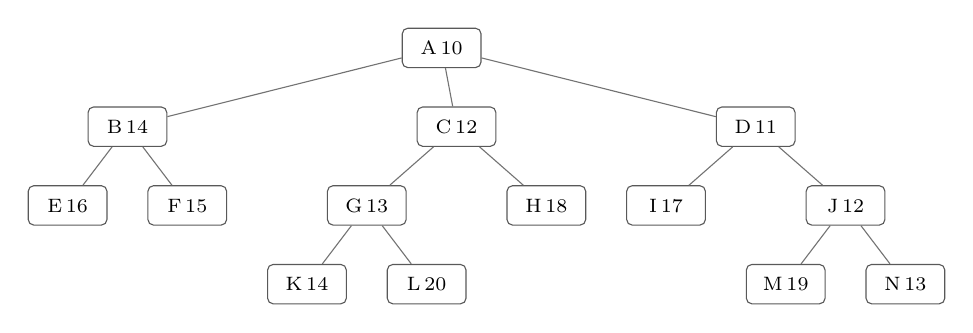
\begin{tikzpicture}[x=1.6cm,y=1cm,
    bt-sbox/.append style={font=\scriptsize, minimum width=1.0cm, minimum height=0.5cm}]
\node[bt-sbox] (a1) at (2.969,0.0) {A\,10};
\node[bt-sbox] (a2) at (0.475,-1.0) {B\,14};
\node[bt-sbox] (a3) at (3.087,-1.0) {C\,12};
\node[bt-sbox] (a4) at (5.462,-1.0) {D\,11};
\node[bt-sbox] (a5) at (0.0,-2.0) {E\,16};
\node[bt-sbox] (a6) at (0.95,-2.0) {F\,15};
\node[bt-sbox] (a7) at (2.375,-2.0) {G\,13};
\node[bt-sbox] (a8) at (3.8,-2.0) {H\,18};
\node[bt-sbox] (a9) at (4.75,-2.0) {I\,17};
\node[bt-sbox] (a10) at (6.175,-2.0) {J\,12};
\node[bt-sbox] (a11) at (1.9,-3.0) {K\,14};
\node[bt-sbox] (a12) at (2.85,-3.0) {L\,20};
\node[bt-sbox] (a13) at (5.7,-3.0) {M\,19};
\node[bt-sbox] (a14) at (6.65,-3.0) {N\,13};
\draw[bt-e] (a1) -- (a2);
\draw[bt-e] (a1) -- (a3);
\draw[bt-e] (a1) -- (a4);
\draw[bt-e] (a2) -- (a5);
\draw[bt-e] (a2) -- (a6);
\draw[bt-e] (a3) -- (a7);
\draw[bt-e] (a3) -- (a8);
\draw[bt-e] (a4) -- (a9);
\draw[bt-e] (a4) -- (a10);
\draw[bt-e] (a7) -- (a11);
\draw[bt-e] (a7) -- (a12);
\draw[bt-e] (a10) -- (a13);
\draw[bt-e] (a10) -- (a14);
\end{tikzpicture}
\end{center}

\item （設計）\textbf{哈密頓環}問題：給一個無向圖，問有沒有一個環恰好經過每個頂點一次。 用
回溯寫出找出所有哈密頓環的虛擬碼（固定從頂點 1 出發），說明顯式限制、隱式限制和你的界限
函數。 每個環會被找到幾次？ 怎麼讓每個環只出現一次？
\end{enumerate}

\section{歷屆試題}
\label{sec:bk-pastexam}

以下是研究所入學考試的原題，題目照原卷（語言、記號、配分照錄）。 詳解在本章最後。

\begin{pastexam}[label={px:bk-1}]{臺大資工所 112 學年度 第 9 題}
［本卷說明：本題為複選題，5 分，每個選項單獨計分。］

\textbf{DFS advantages:} To find a feasible solution to the eight-queen problem, what is/are the reason(s) that we prefer to use DFS (depth-first search) instead of BFS (breadth-first search)?
\begin{enumerate}[label=(\Alph*)]
\item DFS is more memory efficient.
\item DFS can be implemented using a stack.
\item DFS usually reaches the terminal states of "good" or "bad" faster.
\item DFS is conceptually simpler than BFS.
\item BFS cannot be implemented using a stack.
\end{enumerate}
\end{pastexam}

\begin{pastexam}[label={px:bk-2}]{中山資工所 111 學年度 第 1 題（節錄 (b) 小題）}
What are printed by each of the following C program?
\begin{enumerate}[label=(\alph*),start=2]
\item (10\%)
\begin{minted}[fontsize=\small, style=perldoc]{cpp}
void g(char a[ ], int k, int m)
{
    if (k == m) {
        for (int i = 0; i <= m; i++) cout << a[i] << " ";
            cout << endl;
    }
    else
        for (int i = k; i <= m; i++) {
           swap(a[k], a[i]); // exchange
           g(a, k+1, m);
           swap(a[k], a[i]);
        }
}
int main( )
{
    char a[ ]="abcde";
    g(a,0,2);
}
\end{minted}
\end{enumerate}
\end{pastexam}

\begin{pastexam}[label={px:bk-3}]{臺大生機所 111 學年度 第 2 題}
(15\%) Given a graph, write a pseudocode function that colors the graph's vertices such that no two adjacent vertices share the same color by minimizing the total number of colors used.
\end{pastexam}

\begin{pastexam}[label={px:bk-4}]{中興資工所 115 學年度 第 7 題}
［本卷說明：單選題，每題 2 分。］

Branch and Bound differs from backtracking by
\begin{enumerate}[label=\Alph*.,nosep]
\item Using bounds to prune search space
\item Random selection
\item Depth-only search
\item Greedy choices
\end{enumerate}
\end{pastexam}

\begin{pastexam}[label={px:bk-5}]{中央資工所 100 學年度 第 6 題}
Below are the inputs of an instance of the 0/1 knapsack problem with n=5 items and the knapsack capacity M=38. Note that P$_\mathrm{i}$ is the profit of item i and W$_\mathrm{i}$ is the weight of item i, i=1,\ldots,5. The 0/1 knapsack problem is to maximize the total profit of items that are wholly put into the knapsack under the constraint that their total weight should not exceed the knapsack capacity.
\begin{center}
\begin{tabular}{cccccc}
i & 1 & 2 & 3 & 4 & 5 \\
P$_\mathrm{i}$ & 6 & 10 & 4 & 5 & 6 \\
W$_\mathrm{i}$ & 10 & 19 & 8 & 10 & 12 \\
\end{tabular}\\[2pt]
(P$_\mathrm{i}$/W$_\mathrm{i}\ge$ P$_\mathrm{i+1}$/W$_\mathrm{i+1}$)
\end{center}
The problem can be solved by the branch-and-bound strategy on the basis of the best-first search scheme by deriving the lower bound and upper bound for each node in the search tree.
\begin{enumerate}[itemsep=2pt,topsep=2pt]
\item[6.1] (12\%) Derive the upper bound and the lower bound for the root node and explain how you obtain the bounds.
\item[6.2] (6\%) Explain how the bounds can be used in the branch-and-bound strategy. (6\%)
\end{enumerate}
\end{pastexam}

\section{實作練習}
\label{sec:bk-practice}

下面是 Aki-Judge 上和本章相關的題目。 這幾題原本是給《C 程式設計基礎》遞迴章練習用的，資
料量都很小，重點在把狀態空間樹想清楚、把剪枝的條件寫對，正好用來練這一章的技巧。

\begin{center}
\begin{tabular}{llc}
\toprule
小節 & 題目 & 難度 \\
\midrule
排列樹與限制 & \akiref{presentation-orders-within-time-windows}{限定時段的報告順序} & 暖身 \\
 & \akiref{palindrome-free-letter-arrangements}{不含回文的字母卡排列} & 基本 \\
圖著色 & \akiref{exam-slots-with-room-limits}{有容量上限的考試時段安排} & 基本 \\
組合與剪枝 & \akiref{project-team-with-skill-quotas}{技能有人數門檻的專題小組} & 基本 \\
 & \akiref{kit-combinations-that-use-everything}{剛好用完的零件包組合} & 基本 \\
分組 & \akiref{teams-balanced-on-two-skills}{兩種能力都要顧的分組} & 基本 \\
\bottomrule
\end{tabular}
\end{center}

幾題的提示：「限定時段的報告順序」依時段一個一個決定由哪一組上台，時段不在那一組範圍內的
就不是子節點；組別由小到大試，輸出自然是字典序。 「不含回文的字母卡排列」用每個字母還剩幾
張的計數表挑字母，相同的字母在同一層只試一次，就不會產生重複的排列；只要檢查新放的字母
和前一格、前兩格都不同，因為任何一段回文的正中間一定是長度 $2$ 或 $3$ 的回文。 「有容量上
限的考試時段安排」就是第~\ref{sec:bk-coloring}~節的 $m$ 著色，每個時段多一個容量的檢查；
時段由小到大試，第一個找到的就是字典序最小的。 「技能有人數門檻的專題小組」把人數由小到大
試，固定人數時依編號遞增挑人，合不來的兩人當作可行性剪枝。 「剛好用完的零件包組合」和子
集合和很像，但每種零件包可以拿很多次：規定只能用編號不小於上一包的零件包，同一個組合就不
會算很多次；任何一種零件的需求變成負數就剪掉。 這題規定不能寫迴圈，「試下一種零件包」也
要寫成遞迴。 「兩種能力都要顧的分組」讓每位同學加入已經開的組或開一個新組（一次只能開下
一個編號的組，消掉組的編號互換造成的對稱），剩下的人數不夠把組數補滿時就剪掉。

\section{讀完你應該會}
\label{sec:bk-checklist}

\begin{itemize}
\item 能替一個問題寫出解向量、顯式限制和隱式限制，畫出它的狀態空間樹，說出活節點、E-節點、
死節點的意思。
\item 能依產生的順序畫出 4 皇后、子集合和、圖著色的回溯過程，標出被剪掉的節點和答案節點。
\item 能分辨可行性剪枝和界限剪枝，對 0/1 背包寫出分數背包上界，並說明它為什麼不會估得太小。
\item 能用 FIFO、LIFO、LC 三種順序做分支限界，手算 0/1 背包的最佳優先樹，列出 E-節點的順序。
\item 能縮減 TSP 的成本矩陣，算出每個子節點的 $\hat c$，完成一次 LC 分支限界的手算追蹤。
\end{itemize}

\textbf{延伸閱讀}（書末會整理完整的參考資料）

\begin{itemize}
\item Ellis Horowitz、Sartaj Sahni、Sanguthevar Rajasekaran，\textit{Computer
Algorithms}：回溯與分支限界各一章，狀態空間樹的名詞、子集合和的兩個剪枝條件、縮減矩陣的
TSP 都在這兩章。
\item Richard E. Neapolitan，\textit{Foundations of Algorithms}，第 5 版，第 5、6 章：用很多
小例子講回溯和分支限界，0/1 背包的最佳優先搜尋寫得很仔細。
\item Steven S. Skiena，\textit{The Algorithm Design Manual}，第 3 版，第 9 章：從實作的角度
講回溯和剪枝，例子偏向實務。
\item John D. C. Little、Katta G. Murty、Dura W. Sweeney、Caroline Karel，``An Algorithm for the
Traveling Salesman Problem''，\textit{Operations Research} 11(6)，1963：用縮減矩陣做 TSP 分支
限界的原始論文。
\end{itemize}

\addcontentsline{toc}{section}{觀念題解答}
\section*{觀念題解答}

\begin{enumerate}
\item (b)、(c)、(e) 正確。 (a)：界限函數能剪掉多少要看輸入。 例如 $m$ 著色時，如果圖沒有任何邊，每個節點都通過檢查，產生的節點就是整棵狀態空間樹。 (d)：第一個產生的答案節點只代表找到一個上界；
例如它的成本是 $70$，而另一個活節點的 $\hat c = 60$，底下可能有成本 $62$ 的答案。 要等到下
一個 E-節點的 $\hat c$ 不小於 $\mathit{upper}$ 才能停。 (e)：最佳優先搜尋要把活節點都留在佇
列裡，回溯只需要一條路徑。

\item 總和 $52$。 一共產生 $20$ 個節點，三個答案節點依序是 $\{3, 5, 11\}$（節點 5）、
$\{5, 14\}$（節點 14）、$\{7, 12\}$（節點 18）。 左子樹（選 $3$）：節點 2 $(3, 49)$~$\to$~3 $(8, 44)$
$\to$~不選 $7$ 的 4 $(8, 37)$~$\to$~選 $11$ 得答案節點 5；節點 2 不選 $5$ 的 6 $(3, 44)$~$\to$~7 $(3, 37)$~$\to$~8
$(3, 26)$ 是死路（選 $12$ 後再加 $14$ 超過，不選 $12$ 時 $3 + 26 - 12 = 17 < 19$）。 右子樹（不選
$3$）：9 $(0, 49)$~$\to$~10 $(5, 44)$~$\to$~11 $(5, 37)$~$\to$~12 $(5, 26)$~$\to$~13 $(5, 14)$~$\to$~答案節點 14；9 的
右子節點 15 $(0, 44)$~$\to$~16 $(7, 37)$~$\to$~17 $(7, 26)$~$\to$~答案節點 18；15 的右子節點 19 $(0, 37)$~$\to$~20
$(0, 26)$ 是死路。 用範例~\ref{ex:bk-subsets} 跑輸入 \texttt{6 19} 和 \texttt{3 5 7 11 12 14}，
印出同樣三組答案和 \texttt{solutions = 3, nodes = 20}。

\item 在決定 $w_k$ 的節點，已選的和是 $s$，剩下 $w_k, \ldots, w_n$ 的和是 $r$，而且
$w_k \le w_{k+1} \le \cdots \le w_n$。
\begin{itemize}
\item 第 4 行不產生左子節點，是因為 $s + w_k \ne M$ 且 $s + w_k + w_{k+1} > M$。 左子節點的子
樹裡，每個答案都已經選了 $w_k$，和是 $s + w_k$ 再加上 $w_{k+1}, \ldots, w_n$ 裡選的數。 什
麼都不選，和是 $s + w_k \ne M$；至少選一個，選的數都不小於 $w_{k+1}$，和至少
$s + w_k + w_{k+1} > M$。 兩種都不是答案。
\item 第 7 行不產生右子節點，是因為 $s + r - w_k < M$ 或 $s + w_{k+1} > M$。 右子節點的子樹裡，
每個答案的和是 $s$ 加上 $w_{k+1}, \ldots, w_n$ 裡選的數。 前者表示全選也只有 $s + r - w_k <
M$。 後者表示只要選一個就超過 $M$；一個都不選，和是 $s$，而能走到這個節點代表
$s + w_k \le M$，$s < M$，也不是答案。
\end{itemize}
沒排序的例子：$w = \langle 4, 6, 1 \rangle$、$M = 5$，答案是 $\{4, 1\}$。 第一次呼叫
$(s, k, r) = (0, 1, 11)$：$0 + 4 \ne 5$，$0 + 4 + 6 = 10 > 5$，左子節點不產生；右子節點要
$0 + 6 \le 5$，也不產生。 程序什麼都沒找到。

\item
\begin{enumerate}
\item 頂點 1 塗 $1$；頂點 2 不能是 $1$，塗 $2$；頂點 3 的鄰居只有 2 塗過，塗 $1$；頂點 4 不
能和 3 同色，塗 $2$；頂點 5 的鄰居 4、1 分別是 $2$、$1$，塗 $3$。 第一種塗法是
$(1, 2, 1, 2, 3)$，沒有退回過。
\item 一共 $30$ 種；固定頂點 1 塗 $1$ 時 $10$ 種。 數法：固定頂點 1 塗 $1$，頂點 2、3、4 依
序只要和前一個不同，各有 $2$ 種，共 $8$ 種：$(2,1,2)$、$(2,1,3)$、$(2,3,1)$、$(2,3,2)$、
$(3,1,2)$、$(3,1,3)$、$(3,2,1)$、$(3,2,3)$。 頂點 5 要和頂點 4、頂點 1 都不同：頂點 4 塗 $1$
的 $2$ 種，頂點 5 有 $2$ 種選擇；其他 $6$ 種，頂點 5 只剩 $1$ 種。 共 $2 \cdot 2 + 6 \cdot 1 = 10$
種，頂點 1 有 $3$ 種顏色，全部是 $30$ 種。
\item 兩種顏色時，沿著環走，顏色必須 $1, 2, 1, 2, \ldots$ 交替，第 5 個頂點是 $1$，和頂點 1
相鄰卻同色。 長度是奇數的環都不能用兩種顏色塗。
\end{enumerate}

\item 根的上界：$49 + 18 = 67$（重 $10$），剩 $6$ 放物品 3 的 $6/7$，$35 \cdot 6 / 7 = 30$，
共 $97$。 各節點的 $(P, \mathit{Wt}, b)$：2 $(49, 7, 97)$、3 $(0, 0, 73)$；展開 2 得 4 $(67, 10, 97)$、
5 $(49, 7, 92)$；展開 4 得 6（拿物品 3，重 $17$，超重）、7 $(67, 10, 87)$；展開 5 得 8 $(84, 14,
92)$、9 $(49, 7, 69)$ 死；展開 8 得 10（重 $19$，超重）、11 $(84, 14, 84)$ 死；展開 7 得 12 $(87,
15, 87)$，$\mathit{best} = 87$，13 $(67, 10, 67)$ 死；最後取出節點 3 時 $73 \le 87$，丟掉。 E-節點
的順序是 1、2、4、5、8、7：節點 5、8 的上界 $92$ 都比節點 7 的 $87$ 大，所以先展開。 最佳解
是物品 1、2、4，總重 $15$，價值 $87$，共產生 $13$ 個節點；把範例~\ref{ex:bk-knapsack-bb} 的輸入
換成這組資料，程式印出同樣的 E-節點順序。

\item
\begin{enumerate}
\item 列縮減減去 $4$、$6$、$2$、$3$，共 $15$；之後第 2 行最小 $9$、第 3 行最小 $3$，第 1、4 行
已有 $0$，共 $12$。 根的 $\hat c = 27$，縮減後的矩陣：
\[
\begin{array}{c|cccc}
 & 1 & 2 & 3 & 4 \\ \hline
1 & \infty & 0 & 0 & 0 \\
2 & 0 & \infty & 3 & 7 \\
3 & 9 & 0 & \infty & 0 \\
4 & 0 & 2 & 5 & \infty
\end{array}
\]
\item 節點 1 的子節點：節點 2（$1 \to 2$）：$A[1][2] = 0$，第 2 列減 $3$，$\hat c = 27 + 0 + 3 =
30$；節點 3（$1 \to 3$）：$A[1][3] = 0$，不用減，$\hat c = 27$；節點 4（$1 \to 4$）：
$A[1][4] = 0$，第 4 列減 $2$、第 3 行減 $3$，$\hat c = 32$。 展開節點 3（$27$）：節點 5
（$1 \to 3 \to 2$）：$A[3][2] = 0$，第 2 列減 $7$，$\hat c = 34$；節點 6（$1 \to 3 \to 4$）：
$A[3][4] = 0$，第 4 列減 $2$，$\hat c = 29$。 展開節點 6（$29$）：唯一的子節點 7 是葉節點
$1 \to 3 \to 4 \to 2 \to 1$，$\hat c = 29$，$\mathit{upper} \gets 29$。 下一個最小的活節點是
節點 2（$30$），$30 \ge 29$，停止。 E-節點的順序是 1、3、6，最佳路線
$1 \to 3 \to 4 \to 2 \to 1$，成本 $7 + 2 + 14 + 6 = 29$。 根的下界 $27$ 比答案小 $2$，下界不一定
是緊的。
\end{enumerate}

\item FIFO：A、B、C、D、E、F、G。 LIFO：A、D、J、N、M、I、C（A 產生 B、C、D 後取最後放入
的 D；D 產生 I、J 後取 J；J 的子節點 M、N 取 N，再取 M，再取 I，然後才輪到 C）。 LC：A、D、
C、J、G、N、B。 LC 的過程：A 之後活節點是 B(14)、C(12)、D(11)，取 D；加入 I(17)、J(12)，
C 和 J 都是 $12$，C 先產生，取 C；加入 G(13)、H(18)，取 J(12)；加入 M(19)、N(13)，G 和 N 都是
$13$，取先產生的 G；加入 K(14)、L(20)，取 N(13)；剩下最小的是 B 和 K，都是 $14$，取先產生的
B。

\item 解向量 $(x_1, \ldots, x_n)$ 是頂點的走訪順序，$x_1 = 1$。 顯式限制：$x_k \in \{2, \ldots,
n\}$。 隱式限制：$x_2, \ldots, x_n$ 互不相同；$\{x_{k-1}, x_k\}$ 是邊；$\{x_n, x_1\}$ 也是邊。
界限函數在放 $x_k = v$ 時檢查 $v$ 還沒用過、和 $x_{k-1}$ 相鄰；$k = n$ 時另外檢查 $v$ 和頂點
1 相鄰。
寫成和 \proc{Queens} 一樣的形狀。 先設 $x_1 \gets 1$、把頂點 1 標成用過，再呼叫
\proc{Hamiltonian}$(2)$：
\begin{pseudo}[unbreakable]{觀念題 8 的解答}
\Procedure{Hamiltonian}{$k$}
    \For{$v \gets 2$ \To $n$}
        \If{$\mathit{used}[v] = \FALSE$ \AND $\{x_{k-1}, v\} \in E$}
            \State $x_k \gets v$；$\mathit{used}[v] \gets \TRUE$
            \If{$k < n$}
                \State \Call{Hamiltonian}{$k + 1$}
            \ElsIf{$\{v, 1\} \in E$ \AND $x_2 < x_n$}
                \State 輸出 $(x_1, \ldots, x_n)$
            \EndIf
            \State $\mathit{used}[v] \gets \FALSE$ \Comment{撤銷}
        \EndIf
    \EndFor
\EndProcedure
\end{pseudo}
第 3 行就是界限函數。 固定從頂點 1 出發之後，同一個環還會以兩個方向各被找到一次
（$1 \to a \to \cdots \to b \to 1$ 和 $1 \to b \to \cdots \to a \to 1$）；第 7 行多檢查
$x_2 < x_n$，每個環就只出現一次。 還可以加一個界限：每個還沒用過的頂點 $u$ 在環上需要一個前
一站和一個下一站，前一站只能是還沒用過的頂點或目前的尾端 $x_k$，下一站只能是還沒用過的頂點
或頂點 1；所以 $u$ 在「還沒用過的頂點、$x_k$、頂點 1」之中的鄰居如果少於兩個，就可以剪掉。
\end{enumerate}

\addcontentsline{toc}{section}{歷屆試題詳解}
\section*{歷屆試題詳解}

\pastsol{px:bk-1}{臺大資工所 112 學年度 第 9 題}
本書的答案是 \textbf{(A)、(C)}。 題目問的是「偏好 DFS 的理由」，所以一個選項要算對，必須
是正確的敘述，而且真的是 DFS 在八皇后上勝過 BFS 的原因。

先用數字看兩種走法的差別。 狀態空間樹用第~\ref{sec:bk-queens}~節的排列樹，對角線衝突的節點
一產生就剪掉，節點照產生的順序數（被剪掉的也算）。 八皇后的答案全部在第 $8$ 層（放完 $8$ 個皇
后）。 用程式數出各層通過檢查的節點數：

\begin{center}
\begin{tabular}{l*{8}{r}}
\toprule
層 & 1 & 2 & 3 & 4 & 5 & 6 & 7 & 8 \\
\midrule
通過檢查的節點 & 8 & 42 & 140 & 344 & 568 & 550 & 312 & 92 \\
\bottomrule
\end{tabular}
\end{center}

\begin{itemize}
\item DFS（回溯，範例~\ref{ex:bk-nqueens}）：第一組解是第 $337$ 個產生的節點。 任何時刻只需
要記住從根到目前節點的一條路徑，最多 $8$ 層。
\item BFS（FIFO，同樣的剪枝）：第 $8$ 層的節點要等第 $1$ 到 $6$ 層的節點全部展開、第 $7$ 層
也開始展開之後才會出現。 第一組解是第 $5209$ 個產生的節點，佇列裡同時存放的活節點最多
$573$ 個。
\end{itemize}

逐項看：
\begin{itemize}
\item (A) 對。 DFS 只存一條路徑（深度 $8$ 的遞迴，加上欄和對角線的記號陣列）；BFS 要把整層的
活節點放在佇列裡，上面算出最多 $573$ 個。 一般來說，深度 $d$、每個節點最多 $b$ 個子節點的樹，
DFS 要 $O(d)$ 個節點的空間，BFS 最壞要 $O(b^d)$ 個。
\item (B) 敘述本身是對的（第~\ref{sec:sq-recursion}~節：遞迴就是用堆疊實作），但不是偏好 DFS 的理
由：BFS 也一樣能用佇列實作，用哪一種容器本身沒有好壞。
\item (C) 對。 八皇后的解都在第 $8$ 層，DFS 一路往下走，很快就碰到「放滿 $8$ 個」或「這條路走
不下去」的節點，找到第一組解只產生 $337$ 個節點；BFS 要先把淺層全部走完，產生 $5209$ 個節點
才碰到第一組解。
\item (D) 錯。 「概念比較簡單」是主觀的說法，兩者一樣簡單，不是選 DFS 的理由。
\item (E) 錯。 BFS 需要先進先出的佇列，而佇列可以用兩個堆疊做出來：放入時推進第一個堆疊；取
出時，如果第二個堆疊是空的，先把第一個堆疊的元素全部彈出、依序推進第二個堆疊，再從第二個堆
疊彈出。 所以 BFS 也能用堆疊實作；何況這也不是偏好 DFS 的理由。
\end{itemize}

\pastsol{px:bk-2}{中山資工所 111 學年度 第 1 題（節錄 (b) 小題）}
這是《C 程式設計基礎》第~15~章 15.15 節「用交換產生所有排列」的寫法（C++ 的 \texttt{swap}
交換兩個字元，\texttt{cout} 輸出）。 \texttt{g(a, k, m)} 負責決定 \texttt{a[k]}：依序把
\texttt{a[k..m]} 的每一個字元換到第 \texttt{k} 格，遞迴決定後面的格子，回來後再換回去
（撤銷）。 \texttt{m = 2}，所以只排列前三個字元 \texttt{a}、\texttt{b}、\texttt{c}，
\texttt{d}、\texttt{e} 不會被動到，也不會印出。 另外注意縮排：\texttt{cout << endl;} 不在
\texttt{for} 裡面（那個 \texttt{for} 只有一個敘述），所以每個排列印完才換一次行。

遞迴的過程（第~\ref{sec:bk-tree}~節的狀態空間樹，深度 $k$ 決定 \texttt{a[k]}）：

\begin{center}
\begin{tabular}{lll}
\toprule
呼叫 & 這一層的交換 & 結果 \\
\midrule
\texttt{g(0)}，陣列 \texttt{abc} & $i = 0$：不變，\texttt{abc} & 進入 \texttt{g(1)} \\
\quad \texttt{g(1)}，\texttt{abc} & $i = 1$：不變 & \texttt{g(2)} 印 \texttt{a b c} \\
 & $i = 2$：交換 \texttt{a[1]}、\texttt{a[2]}，\texttt{acb} & \texttt{g(2)} 印 \texttt{a c b}，換回 \texttt{abc} \\
\texttt{g(0)} & $i = 1$：交換 \texttt{a[0]}、\texttt{a[1]}，\texttt{bac} & 進入 \texttt{g(1)} \\
\quad \texttt{g(1)}，\texttt{bac} & $i = 1$：不變 & 印 \texttt{b a c} \\
 & $i = 2$：\texttt{bca} & 印 \texttt{b c a}，換回 \texttt{bac} \\
\texttt{g(0)} & 換回 \texttt{abc}；$i = 2$：交換 \texttt{a[0]}、\texttt{a[2]}，\texttt{cba} & 進入 \texttt{g(1)} \\
\quad \texttt{g(1)}，\texttt{cba} & $i = 1$：不變 & 印 \texttt{c b a} \\
 & $i = 2$：\texttt{cab} & 印 \texttt{c a b}，換回 \texttt{cba} \\
\texttt{g(0)} & 換回 \texttt{abc} & 結束 \\
\bottomrule
\end{tabular}
\end{center}

輸出六行（每個字元後面都有一個空白）：

\noindent\begin{minipage}{\linewidth}
\begin{verbatim}
a b c
a c b
b a c
b c a
c b a
c a b
\end{verbatim}
\end{minipage}
最後兩行是 \texttt{c b a} 在 \texttt{c a b} 前面，不是字典序：第三輪把 \texttt{a[0]} 和
\texttt{a[2]} 交換，得到的是 \texttt{cba}，第 1、2 格的順序也跟著變了。 一共呼叫 \texttt{g}
$1 + 3 + 6 = 10$ 次，正是 $3$ 個元素的排列樹的節點數。

\pastsol{px:bk-3}{臺大生機所 111 學年度 第 2 題}
用的顏色越少越好，就是求圖的色數（第~\ref{sec:bk-coloring}~節）。 做法：依序試
$m = 1, 2, 3, \ldots$，每個 $m$ 用回溯檢查「能不能用 $m$ 種顏色塗」，第一個成功的 $m$ 就是最少
的顏色數。 回溯就是虛擬碼~\ref{alg:bk-color}，改成找到第一種塗法就停。 頂點編號 $1$ 到 $n$
（$n \ge 1$），$x_i$ 是頂點 $i$ 的顏色，$\mathit{found}$ 是全域的旗標。

\begin{pseudo}[unbreakable]{用最少顏色著色}
\Procedure{Try-Color}{$k, m$} \Comment{頂點 $1..k-1$ 已經塗好}
    \For{$c \gets 1$ \To $m$}
        \If{$k$ 的每個鄰居 $j < k$ 都有 $x_j \ne c$}
            \State $x_k \gets c$
            \If{$k = n$}
                \State $\mathit{found} \gets \TRUE$
            \Else
                \State \Call{Try-Color}{$k + 1, m$}
            \EndIf
            \If{$\mathit{found}$}
                \State \Return \Comment{找到一種塗法就不再試別的顏色}
            \EndIf
        \EndIf
    \EndFor
\EndProcedure
\Statex
\Function{Min-Coloring}{$G$}
    \For{$m \gets 1$ \To $n$}
        \State $\mathit{found} \gets \FALSE$
        \State \Call{Try-Color}{$1, m$}
        \If{$\mathit{found}$}
            \State \Return $m$ 和塗法 $(x_1, \ldots, x_n)$
        \EndIf
    \EndFor
\EndFunction
\end{pseudo}

\textbf{正確性。} \proc{Try-Color}$(1, m)$ 走的是 $m$ 著色的狀態空間樹，只剪掉「新塗的頂點和
已經塗過的鄰居同色」的節點，這種節點不管後面怎麼塗都有一條邊兩端同色，子樹裡沒有合法的塗
法。 其他節點都會被走到（除非已經找到），所以 $\mathit{found}$ 變成 \TRUE{} 若且唯若圖能用
$m$ 種顏色塗，而且那時 $x_1, \ldots, x_n$ 就是一種合法的塗法。 $m$ 由小到大試，第一個成功的
$m$ 之前每一個都不能塗，所以它就是最少的顏色數。 $m = n$ 時每個頂點一種顏色一定可以，所以
迴圈一定會回傳。

\textbf{時間。} 對固定的 $m$，狀態空間樹最多 $\sum_{i=0}^{n} m^i = O(m^n)$ 個節點，用鄰接串
列檢查第 3 行，每個節點 $O(n)$，所以一次 \proc{Try-Color}$(1, m)$ 是 $O(n m^n)$。 設最少要
$\chi$ 種顏色，總時間是 $\sum_{m=1}^{\chi} O(n m^n) = O(n \chi^{n+1})$，最壞是指數時間。 這
個問題的決策版本在 $m \ge 3$ 時是 NP 完備的（第~28~章），目前沒有已知的多項式時間演算法；
實務上可以用第~\ref{sec:bk-coloring}~節的「固定頂點 1 塗顏色 $1$」去掉對稱，先塗鄰居多的頂
點，讓搜尋少走一些節點。

\textbf{不要寫成單純的貪心。} 「每個頂點依序塗上鄰居沒用過的最小顏色」只要
$O(n + m_E)$（$m_E$ 是邊數），塗出來一定合法，但顏色不一定最少。 例如四個頂點、邊
$\{1, 3\}$、$\{3, 4\}$、$\{4, 2\}$（一條路徑 $1 - 3 - 4 - 2$）：依編號塗，頂點 1、2 都塗 $1$，
頂點 3 塗 $2$，頂點 4 的鄰居用了 $1$、$2$，只好塗 $3$；其實兩種顏色就夠（$1$、$4$ 一色，
$2$、$3$ 另一色）。 題目要求最少，所以要用上面的搜尋；用 \proc{Min-Coloring} 算這個圖，
$m = 2$ 就成功。

\pastsol{px:bk-4}{中興資工所 115 學年度 第 7 題}
答案是 \textbf{A}。

嚴格說，回溯也會用界限函數剪枝（第~\ref{sec:bk-tree}~節），所以 A 要理解成分支限界的特色：
它通常用來解最佳化問題，對每個節點算出目標值的上界或下界，和目前找到的最好解比較，不可能更
好的子樹整棵丟掉（第~\ref{sec:bk-bb}~節的界限剪枝）；而且 E-節點一次產生全部的子節點，再依
FIFO、LIFO 或最小成本挑下一個 E-節點。 四個選項裡只有 A 說的是分支限界。

\begin{itemize}
\item B 錯：分支限界挑下一個 E-節點的規則是固定的（佇列、堆疊或 $\hat c$ 最小），不是隨機。
\item C 錯：只往深處走是回溯的走法；分支限界可以一層一層走（FIFO），也可以照界限跳來跳去（最
佳優先）。
\item D 錯：貪心一旦做了選擇就不再回頭；分支限界把其他活節點都留著，之後還可能回去展開。 例
如第~\ref{sec:bk-tsp}~節的 TSP，展開節點 6 之後又跳回第 1 層展開節點 2。
\end{itemize}

\pastsol{px:bk-5}{中央資工所 100 學年度 第 6 題}
物品已經依 $P_i / W_i$ 由大到小排好：$0.6, 0.526\ldots, 0.5, 0.5, 0.5$。

\textbf{6.1 上界。} 用第~\ref{sec:bk-knap}~節的分數背包上界（虛擬碼~\ref{alg:bk-bound}）：
把物品照順序放，放得下就整個放，放不下的那一個只放剛好填滿的部分。

\begin{center}
\begin{tabular}{cccl}
\toprule
物品 & 放進去的部分 & 累計重量 & 累計價值 \\
\midrule
1 & 整個 & 10 & 6 \\
2 & 整個 & 29 & 16 \\
3 & 整個 & 37 & 20 \\
4 & 剩下容量 $1$，放 $1/10$ & 38 & $20 + 5 \cdot \frac{1}{10} = 20.5$ \\
\bottomrule
\end{tabular}
\end{center}

上界是 $20.5$。 理由：任何一個 0/1 的解也是同一組資料的分數背包的解，而上面的貪心解是分數背
包的最佳解（定理~\ref{thm:gr-frac}），所以每個 0/1 的解價值都不超過 $20.5$。 價值都是整數，
上界可以再收緊成 $\lfloor 20.5 \rfloor = 20$。

\textbf{6.1 下界。} 找一個實際放得進去的 0/1 解，它的價值就是最佳值的下界。 用同樣的順序做
整數的貪心：物品 1、2、3 放得下（重 $37$），物品 4 放進去會變成 $47 > 38$，跳過；物品 5 放進
去是 $49 > 38$，也跳過。 得到 $\{1, 2, 3\}$，價值 $20$，所以下界是 $20$。

\textbf{6.2 界限怎麼用。} 用最佳優先的分支限界（第~\ref{sec:bk-knap}~節）：
\begin{enumerate}
\item 每個節點代表「前 $k$ 個物品已經決定拿或不拿」，算出它的上界（這棵子樹裡的解最多值多少）
和下界（這棵子樹裡一定做得到的值）。
\item 記住目前所有節點裡最大的下界 $\mathit{best}$，它是某個實際的解。
\item 每次從活節點裡取上界最大的展開，產生「拿」和「不拿」兩個子節點；超重的子節點丟掉。
\item 上界 $\le \mathit{best}$ 的節點不必展開，因為它的子樹裡不會有比 $\mathit{best}$ 更好的
解（界限剪枝）。 活節點裡最大的上界都 $\le \mathit{best}$ 時就停止，$\mathit{best}$ 就是最佳值。
\end{enumerate}

用在這一題：根的上界收緊後是 $20$，等於下界 $20$，所以根就停了，$\{1, 2, 3\}$、價值 $20$ 是
最佳解，不必展開任何節點（把 $32$ 種組合全部列出來檢查，最大值也是 $20$）。 如果上界不取整，
照虛擬碼~\ref{alg:bk-knap-bb} 做，$20.5 > 20$ 的節點會一直被展開：要產生 $15$ 個節點、展開 $7$
個 E-節點（依序是 1、2、4、6、7、9、11）才停下，答案同樣是 $20$。 價值是整數時把上界取整，可
以少走很多節點。

有的課本（第~\ref{sec:bk-knap}~節的作答提醒）把背包改寫成求最小值：價值取負號，根的
$\hat c = -20.5$、上界 $u = -20$，$\mathit{upper}$ 從 $-20$ 開始；數字的正負號相反，用法相同。
